\makeatletter \@ifundefined{rootpath}{% Manual to memoir http://mirrors.dotsrc.org/ctan/macros/latex/contrib/memoir/memman.pdf

%\documentclass[a4paper,12pt,fleqn,openany,twoside]{memoir} %two sides for printing
\documentclass[a4paper,12pt,fleqn,openany,oneside]{memoir} %one side for pdf
\usepackage[english]{babel}
\usepackage[utf8]{inputenc}
\usepackage{microtype}
\usepackage{paralist}

%Definitions
\usepackage{amsthm}
\theoremstyle{plain}
\newtheorem{thm}{Theorem}[chapter] % reset theorem numbering for each chapter
\theoremstyle{definition}
\newtheorem{defn}[thm]{Definition}


% Choses the depth of numerations
\setsecnumdepth{subsubsection}

% Choses the depth of toc
%\maxtocdepth{subsection}

% LaTeX logical statements
\usepackage{ifthen}

% Fancy space after use of e.g. command
\usepackage{xspace}

% Skips after paragraphs
\usepackage{parskip}

% Layout settings
\setlength{\parindent}{0cm}
\setlength{\parskip}{2ex plus 2ex} %kan udvides til f.eks: '2ex plus 2ex minus 0ex'

\sloppybottom

% Don't make a collection per default
\newcommand{\worksheetcollection}{false}

% Bibtex
\usepackage[square,numbers,sort,comma]{natbib}
%\usepackage{cite}
%\bibliographystyle{plainnat}
\bibliographystyle{IEEEtran}


% Fixmes
\usepackage{fixme}
\fxsetup{draft}

% Mathematic
\usepackage{amsmath}
\usepackage{amsfonts}
\usepackage{amssymb}
\usepackage{stmaryrd}
\allowdisplaybreaks[1]


% Acronyms
\usepackage[printonlyused]{acronym}

% Images
\usepackage{graphicx}
\usepackage{wrapfig}
\usepackage[outdir=./]{epstopdf}
\usepackage{epsfig}


% Captions ans subcaptions
\captionnamefont{\footnotesize\bfseries}
\captiontitlefont{\footnotesize}

% Enable memoir subfloats for figures and tables
\newsubfloat{figure}
\newsubfloat{table}

% Hack memoir subfigure styles to have bold label and footnotesize fonts
\renewcommand{\thesubfigure}{\footnotesize\bfseries{(\alph{subfigure})}}
\renewcommand{\thesubtable}{\footnotesize\bfseries{(\alph{subtable})}}

\renewcommand{\subcaption}[2][]{\subbottom[\footnotesize{#1}]{#2}}

% Memoir tweak pagenumbers
%\pagestyle{headings}

% Tikz
\usepackage{tikz}
\usetikzlibrary{arrows,shapes,calc,positioning}
\pgfmathsetseed{1}

%Pgf plots
\usepackage{pgfplots}
\pgfplotsset{compat=1.5}
% loatbarrier, keep figures within (sub,subsub) sections
\usepackage{placeins}
\usepackage{pgfplots}
\usepgfplotslibrary{units}
\usepackage[space-before-unit,range-units = repeat]{siunitx}

% Hyperlinked auto references
\usepackage[hidelinks]{hyperref}
\usepackage[nameinlink]{cleveref}
\crefname{lstlisting}{Listing}{Listings}  
\Crefname{lstlisting}{Listing}{Listings}

\crefname{thm}{definition}{definitions}
\Crefname{thm}{Definition}{Definitions}

%\def\chapterautorefname{Kapitel}
%\def\sectionautorefname{Afsnit}
%\def\subsectionautorefname{Afsnit}
%\def\subsubsectionautorefname{Underafsnit}
%\def\figureautorefname{Figur}
%\def\lstlistingautorefname{Listing}
%\def\lstnumberautorefname{Linje}
%\def\itemautorefname{Punkt}
\usepackage[hypcap]{caption} % Link to top of the figure and not the caption

%Sick shit to make \Autoref command
%http://tex.stackexchange.com/questions/36575/autorefs-inserted-text-has-not-the-correct-case
\def\HyLang@english{%
  \def\equationautorefname{Equation}%
  \def\footnoteautorefname{Footnote}%
  \def\itemautorefname{item}%
  \def\figureautorefname{Figure}%
  \def\tableautorefname{Table}%
  \def\partautorefname{Part}%
  \def\appendixautorefname{Appendix}%
  \def\chapterautorefname{Chapter}%
  \def\sectionautorefname{Section}%
  \def\subsectionautorefname{Subsection}%
  \def\subsubsectionautorefname{Subsubsection}%
  \def\paragraphautorefname{Paragraph}%
  \def\subparagraphautorefname{Subparagraph}%
  \def\FancyVerbLineautorefname{Line}%
  \def\theoremautorefname{Theorem}%
  \def\pageautorefname{Page}%
}

% Reference greencommentssections with number and name
\usepackage{nameref}
\newcommand{\bsnameref}[1]{\Cref{#1} ``\nameref{#1}''}
\newcommand{\bsref}[1]{\Cref{#1}}
\newcommand{\bsbilagref}[1]{Appendix \ref{#1}}
\newcommand{\bsbilagnameref}[1]{Appendix \ref{#1} ``\nameref{#1}''}
\newcommand{\pling}[1]{``#1''}


% Listings for code qoutes
\usepackage{listings}
%\usepackage[usenames,dvipsnames,svgnames,table]{xcolor}
\usepackage{color}
\usepackage{xcolor}
\definecolor{bluekeywords}{rgb}{0.13,0.13,1}
\definecolor{greencomments}{rgb}{0,0.5,0}
\definecolor{redstrings}{rgb}{0.9,0,0}
\usepackage{caption} 
\usepackage{multicol}
\DeclareCaptionFont{white}{\color{white}}
\DeclareCaptionFormat{listing}{\colorbox{gray}{\parbox{\textwidth}{#1#2#3}}}
\captionsetup[lstlisting]{format=listing,labelfont=white,textfont=white}
%\lstset{numbers=left}
\lstset{
	basicstyle=\footnotesize,
	tabsize=2,
	breaklines=true,
  literate={æ}{{\ae}}1 {ø}{{\o}}1 {å}{{\aa}}1 {Æ}{{\AE}}1 {Ø}{{\O}}1 {Å}{{\AA}}1,
  keywords={typeof, new, true, false, catch, function, return, null, catch, switch, var, if, in, while, do, else, case, break},
  keywordstyle=\color{blue}\bfseries,
  ndkeywords={class, export, boolean, throw, implements, import, this},
  ndkeywordstyle=\color{darkgray}\bfseries,
  identifierstyle=\color{black},
  sensitive=false,
  comment=[l]{//},
  morecomment=[s]{/*}{*/},
  commentstyle=\color{purple}\ttfamily,
  stringstyle=\color{red}\ttfamily,
  numbers=left,
  numbersep=-5pt,
  showstringspaces=false,
  showspaces=false,
  %morestring=[b]',
  %morestring=[b]"
}
\lstnewenvironment{code}[1][]%
  {\minipage{\linewidth} 
   \lstset{basicstyle=\ttfamily\footnotesize,frame=single,#1}}
  {\endminipage}

\lstdefinelanguage{scala}{
  morekeywords={abstract,case,catch,class,def,%
    do,else,extends,false,final,finally,%
    for,if,implicit,import,match,mixin,%
    new,null,object,override,package,%
    private,protected,requires,return,sealed,%
    super,this,throw,trait,true,try,%
    type,val,var,while,with,yield, Unit, Boolean, Int},
  otherkeywords={=>,<-,<\%,<:,>:,\#,@},
  sensitive=true,
  morecomment=[l]{//},
  morecomment=[n]{/*}{*/},
  morestring=[b]",
  morestring=[b]',
  morestring=[b]"""
}

\lstdefinelanguage{clojure}%
{morekeywords={*,*1,*2,*3,*agent*,*allow-unresolved-vars*,*assert*,*clojure-version*,*command-line-args*,%
*compile-files*,*compile-path*,*e,*err*,*file*,*flush-on-newline*,*in*,*macro-meta*,%
*math-context*,*ns*,*out*,*print-dup*,*print-length*,*print-level*,*print-meta*,*print-readably*,%
*read-eval*,*source-path*,*use-context-classloader*,*warn-on-reflection*,+,-,->,->>,..,/,:else,%
<,<=,=,==,>,>=,@,accessor,aclone,add-classpath,add-watch,agent,agent-errors,aget,alength,alias,%
all-ns,alter,alter-meta!,alter-var-root,amap,ancestors,and,apply,areduce,array-map,aset,%
aset-boolean,aset-byte,aset-char,aset-double,aset-float,aset-int,aset-long,aset-short,assert,%
assoc,assoc!,assoc-in,associative?,atom,await,await-for,await1,bases,bean,bigdec,bigint,binding,%
bit-and,bit-and-not,bit-clear,bit-flip,bit-not,bit-or,bit-set,bit-shift-left,bit-shift-right,%
bit-test,bit-xor,boolean,boolean-array,booleans,bound-fn,bound-fn*,butlast,byte,byte-array,%
bytes,cast,char,char-array,char-escape-string,char-name-string,char?,chars,chunk,chunk-append,%
chunk-buffer,chunk-cons,chunk-first,chunk-next,chunk-rest,chunked-seq?,class,class?,%
clear-agent-errors,clojure-version,coll?,comment,commute,comp,comparator,compare,compare-and-set!,%
compile,complement,concat,cond,condp,conj,conj!,cons,constantly,construct-proxy,contains?,count,%
counted?,create-ns,create-struct,cycle,dec,decimal?,declare,def,definline,defmacro,defmethod,%
defmulti,defn,defn-,defonce,defprotocol,defstruct,deftype,delay,delay?,deliver,deref,derive,%
descendants,destructure,disj,disj!,dissoc,dissoc!,distinct,distinct?,do,do-template,doall,doc,%
dorun,doseq,dosync,dotimes,doto,double,double-array,doubles,drop,drop-last,drop-while,empty,empty?,%
ensure,enumeration-seq,eval,even?,every?,false,false?,ffirst,file-seq,filter,finally,find,find-doc,%
find-ns,find-var,first,float,float-array,float?,floats,flush,fn,fn?,fnext,for,force,format,future,%
future-call,future-cancel,future-cancelled?,future-done?,future?,gen-class,gen-interface,gensym,%
get,get-in,get-method,get-proxy-class,get-thread-bindings,get-validator,hash,hash-map,hash-set,%
identical?,identity,if,if-let,if-not,ifn?,import,in-ns,inc,init-proxy,instance?,int,int-array,%
integer?,interleave,intern,interpose,into,into-array,ints,io!,isa?,iterate,iterator-seq,juxt,%
key,keys,keyword,keyword?,last,lazy-cat,lazy-seq,let,letfn,line-seq,list,list*,list?,load,load-file,%
load-reader,load-string,loaded-libs,locking,long,long-array,longs,loop,macroexpand,macroexpand-1,%
make-array,make-hierarchy,map,map?,mapcat,max,max-key,memfn,memoize,merge,merge-with,meta,%
method-sig,methods,min,min-key,mod,monitor-enter,monitor-exit,name,namespace,neg?,new,newline,%
next,nfirst,nil,nil?,nnext,not,not-any?,not-empty,not-every?,not=,ns,ns-aliases,ns-imports,%
ns-interns,ns-map,ns-name,ns-publics,ns-refers,ns-resolve,ns-unalias,ns-unmap,nth,nthnext,num,%
number?,odd?,or,parents,partial,partition,pcalls,peek,persistent!,pmap,pop,pop!,pop-thread-bindings,%
pos?,pr,pr-str,prefer-method,prefers,primitives-classnames,print,print-ctor,print-doc,print-dup,%
print-method,print-namespace-doc,print-simple,print-special-doc,print-str,printf,println,println-str,%
prn,prn-str,promise,proxy,proxy-call-with-super,proxy-mappings,proxy-name,proxy-super,%
push-thread-bindings,pvalues,quot,rand,rand-int,range,ratio?,rational?,rationalize,re-find,%
re-groups,re-matcher,re-matches,re-pattern,re-seq,read,read-line,read-string,recur,reduce,ref,%
ref-history-count,ref-max-history,ref-min-history,ref-set,refer,refer-clojure,reify,%
release-pending-sends,rem,remove,remove-method,remove-ns,remove-watch,repeat,repeatedly,%
replace,replicate,require,reset!,reset-meta!,resolve,rest,resultset-seq,reverse,reversible?,%
rseq,rsubseq,second,select-keys,send,send-off,seq,seq?,seque,sequence,sequential?,set,set!,%
set-validator!,set?,short,short-array,shorts,shutdown-agents,slurp,some,sort,sort-by,sorted-map,%
sorted-map-by,sorted-set,sorted-set-by,sorted?,special-form-anchor,special-symbol?,split-at,%
split-with,str,stream?,string?,struct,struct-map,subs,subseq,subvec,supers,swap!,symbol,symbol?,%
sync,syntax-symbol-anchor,take,take-last,take-nth,take-while,test,the-ns,throw,time,to-array,%
to-array-2d,trampoline,transient,tree-seq,true,true?,try,type,unchecked-add,unchecked-dec,%
unchecked-divide,unchecked-inc,unchecked-multiply,unchecked-negate,unchecked-remainder,%
unchecked-subtract,underive,unquote,unquote-splicing,update-in,update-proxy,use,val,vals,%
var,var-get,var-set,var?,vary-meta,vec,vector,vector?,when,when-first,when-let,when-not,%
while,with-bindings,with-bindings*,with-in-str,with-loading-context,with-local-vars,%
with-meta,with-open,with-out-str,with-precision,xml-seq,zero?,zipmap
},%
   sensitive,% ???
   alsodigit=-,%
   morecomment=[l];,%
   morestring=[b]"%
  }[keywords,comments,strings]%

% Worksheet commands
\newcommand{\worksheetstart}[5]{ %Title, Revision, Date, Author, rootpath
	\ifthenelse{\equal{\worksheetcollection}{false}}{
		\newcommand{\rootpath}{#5}
		\documentheader
		\chapter{#1}
	}{
		\chapter{#1}
	}
%	\vspace{-1em}
%	\textbf{\tiny Revision #2 at #3. Written by #4}\\
%	\textbf{\tiny Hovedansvarlig #4}\\
%	\vspace{2em}\\
}

\newcommand{\worksheetend}{
	\ifthenelse{\equal{\worksheetcollection}{false}}{
		\collectionend
	}{}
}

\newcommand{\documentheader}{
	% Draws a tikz camera
% #1 is the coordinate to the top left corner
% #2 is a label for the righthand center position
% #3 is the text shown in the center of the camera
\newcommand{\camera}[3]{
\coordinate (anchor) at #1;
\draw (anchor) -- ($ (anchor) + (0em,-20pt) $) -- ($ (anchor) + (10pt, -15pt) $) -- ($ (anchor) + (10pt,-5pt)$) -- cycle;
\draw ($ (anchor) + (10pt,-5pt) $) -- ($ (anchor) + (10pt,0pt) $) -- ($ (anchor) + (50pt,0pt) $) -- ($ (anchor) + (50pt,-20pt) $) -- node[yshift=10pt] {\tiny #3} ($ (anchor) + (10pt,-20pt) $)-- cycle;
\coordinate (#2) at ($ (anchor) + (50pt,-10pt) $);
}

\newcounter{frameNumber}
\newcommand{\frameWithSize}[3][false]{
	\stepcounter{frameNumber}
	\coordinate (anchor) at #2;
	\ifthenelse{\equal{#1}{false}}{
		\def\frameNumber{\arabic{frameNumber}}
	}{
		\def\frameNumber{#1}
	}
	\pgfmathtruncatemacro\randomnumber{random(0,4)}
	\node[yshift=20pt] at (anchor) {\frameNumber};
	\ifthenelse{\equal{#3}{I}}{
		\node[draw, minimum size=20pt, fill=green!60] at (anchor) {I};
		\filldraw[fill=gray] ($(anchor) + (-10pt,-40pt)$) rectangle ($(anchor) + (10pt,-20pt) + (0pt,\randomnumber pt)$);
	}{
		\ifthenelse{\equal{#3}{P}}{
			\node[draw, minimum size=20pt, fill=yellow!60] at (anchor) {P};
			\filldraw[fill=gray] ($(anchor) + (-10pt,-40pt)$) rectangle ($(anchor) + (10pt,-30pt) + (0pt,\randomnumber pt)$);
		}{
			\node[draw, minimum size=20pt, fill=blue!40!yellow!60!black] at (anchor) {\color{white}B};
			\filldraw[fill=gray] ($(anchor) + (-10pt,-40pt)$) rectangle ($(anchor) + (10pt,-37pt) + (0pt,\randomnumber pt)$);
		}
	}
	\draw[thick] ($(anchor) + (-10pt,-40pt)$) -- +(20pt,0pt);
}

	\begin{document}
	%\renewcommand{\chaptername}{Worksheet}
	\chapterstyle{section}
	\renewcommand{\beforechapskip}{0pt}
	\renewcommand{\afterchapskip}{0pt}
}

\newcommand{\collectionstart}[1]{
	\newcommand{\rootpath}{#1}
	\renewcommand{\worksheetcollection}{true}
	\documentheader
	\frontmatter
	%\forside
	\makeatletter \@ifundefined{rootpath}{% Manual to memoir http://mirrors.dotsrc.org/ctan/macros/latex/contrib/memoir/memman.pdf

%\documentclass[a4paper,12pt,fleqn,openany,twoside]{memoir} %two sides for printing
\documentclass[a4paper,12pt,fleqn,openany,oneside]{memoir} %one side for pdf
\usepackage[english]{babel}
\usepackage[utf8]{inputenc}
\usepackage{microtype}
\usepackage{paralist}

%Definitions
\usepackage{amsthm}
\theoremstyle{plain}
\newtheorem{thm}{Theorem}[chapter] % reset theorem numbering for each chapter
\theoremstyle{definition}
\newtheorem{defn}[thm]{Definition}


% Choses the depth of numerations
\setsecnumdepth{subsubsection}

% Choses the depth of toc
%\maxtocdepth{subsection}

% LaTeX logical statements
\usepackage{ifthen}

% Fancy space after use of e.g. command
\usepackage{xspace}

% Skips after paragraphs
\usepackage{parskip}

% Layout settings
\setlength{\parindent}{0cm}
\setlength{\parskip}{2ex plus 2ex} %kan udvides til f.eks: '2ex plus 2ex minus 0ex'

\sloppybottom

% Don't make a collection per default
\newcommand{\worksheetcollection}{false}

% Bibtex
\usepackage[square,numbers,sort,comma]{natbib}
%\usepackage{cite}
%\bibliographystyle{plainnat}
\bibliographystyle{IEEEtran}


% Fixmes
\usepackage{fixme}
\fxsetup{draft}

% Mathematic
\usepackage{amsmath}
\usepackage{amsfonts}
\usepackage{amssymb}
\usepackage{stmaryrd}
\allowdisplaybreaks[1]


% Acronyms
\usepackage[printonlyused]{acronym}

% Images
\usepackage{graphicx}
\usepackage{wrapfig}
\usepackage[outdir=./]{epstopdf}
\usepackage{epsfig}


% Captions ans subcaptions
\captionnamefont{\footnotesize\bfseries}
\captiontitlefont{\footnotesize}

% Enable memoir subfloats for figures and tables
\newsubfloat{figure}
\newsubfloat{table}

% Hack memoir subfigure styles to have bold label and footnotesize fonts
\renewcommand{\thesubfigure}{\footnotesize\bfseries{(\alph{subfigure})}}
\renewcommand{\thesubtable}{\footnotesize\bfseries{(\alph{subtable})}}

\renewcommand{\subcaption}[2][]{\subbottom[\footnotesize{#1}]{#2}}

% Memoir tweak pagenumbers
%\pagestyle{headings}

% Tikz
\usepackage{tikz}
\usetikzlibrary{arrows,shapes,calc,positioning}
\pgfmathsetseed{1}

%Pgf plots
\usepackage{pgfplots}
\pgfplotsset{compat=1.5}
% loatbarrier, keep figures within (sub,subsub) sections
\usepackage{placeins}
\usepackage{pgfplots}
\usepgfplotslibrary{units}
\usepackage[space-before-unit,range-units = repeat]{siunitx}

% Hyperlinked auto references
\usepackage[hidelinks]{hyperref}
\usepackage[nameinlink]{cleveref}
\crefname{lstlisting}{Listing}{Listings}  
\Crefname{lstlisting}{Listing}{Listings}

\crefname{thm}{definition}{definitions}
\Crefname{thm}{Definition}{Definitions}

%\def\chapterautorefname{Kapitel}
%\def\sectionautorefname{Afsnit}
%\def\subsectionautorefname{Afsnit}
%\def\subsubsectionautorefname{Underafsnit}
%\def\figureautorefname{Figur}
%\def\lstlistingautorefname{Listing}
%\def\lstnumberautorefname{Linje}
%\def\itemautorefname{Punkt}
\usepackage[hypcap]{caption} % Link to top of the figure and not the caption

%Sick shit to make \Autoref command
%http://tex.stackexchange.com/questions/36575/autorefs-inserted-text-has-not-the-correct-case
\def\HyLang@english{%
  \def\equationautorefname{Equation}%
  \def\footnoteautorefname{Footnote}%
  \def\itemautorefname{item}%
  \def\figureautorefname{Figure}%
  \def\tableautorefname{Table}%
  \def\partautorefname{Part}%
  \def\appendixautorefname{Appendix}%
  \def\chapterautorefname{Chapter}%
  \def\sectionautorefname{Section}%
  \def\subsectionautorefname{Subsection}%
  \def\subsubsectionautorefname{Subsubsection}%
  \def\paragraphautorefname{Paragraph}%
  \def\subparagraphautorefname{Subparagraph}%
  \def\FancyVerbLineautorefname{Line}%
  \def\theoremautorefname{Theorem}%
  \def\pageautorefname{Page}%
}

% Reference greencommentssections with number and name
\usepackage{nameref}
\newcommand{\bsnameref}[1]{\Cref{#1} ``\nameref{#1}''}
\newcommand{\bsref}[1]{\Cref{#1}}
\newcommand{\bsbilagref}[1]{Appendix \ref{#1}}
\newcommand{\bsbilagnameref}[1]{Appendix \ref{#1} ``\nameref{#1}''}
\newcommand{\pling}[1]{``#1''}


% Listings for code qoutes
\usepackage{listings}
%\usepackage[usenames,dvipsnames,svgnames,table]{xcolor}
\usepackage{color}
\usepackage{xcolor}
\definecolor{bluekeywords}{rgb}{0.13,0.13,1}
\definecolor{greencomments}{rgb}{0,0.5,0}
\definecolor{redstrings}{rgb}{0.9,0,0}
\usepackage{caption} 
\usepackage{multicol}
\DeclareCaptionFont{white}{\color{white}}
\DeclareCaptionFormat{listing}{\colorbox{gray}{\parbox{\textwidth}{#1#2#3}}}
\captionsetup[lstlisting]{format=listing,labelfont=white,textfont=white}
%\lstset{numbers=left}
\lstset{
	basicstyle=\footnotesize,
	tabsize=2,
	breaklines=true,
  literate={æ}{{\ae}}1 {ø}{{\o}}1 {å}{{\aa}}1 {Æ}{{\AE}}1 {Ø}{{\O}}1 {Å}{{\AA}}1,
  keywords={typeof, new, true, false, catch, function, return, null, catch, switch, var, if, in, while, do, else, case, break},
  keywordstyle=\color{blue}\bfseries,
  ndkeywords={class, export, boolean, throw, implements, import, this},
  ndkeywordstyle=\color{darkgray}\bfseries,
  identifierstyle=\color{black},
  sensitive=false,
  comment=[l]{//},
  morecomment=[s]{/*}{*/},
  commentstyle=\color{purple}\ttfamily,
  stringstyle=\color{red}\ttfamily,
  numbers=left,
  numbersep=-5pt,
  showstringspaces=false,
  showspaces=false,
  %morestring=[b]',
  %morestring=[b]"
}
\lstnewenvironment{code}[1][]%
  {\minipage{\linewidth} 
   \lstset{basicstyle=\ttfamily\footnotesize,frame=single,#1}}
  {\endminipage}

\lstdefinelanguage{scala}{
  morekeywords={abstract,case,catch,class,def,%
    do,else,extends,false,final,finally,%
    for,if,implicit,import,match,mixin,%
    new,null,object,override,package,%
    private,protected,requires,return,sealed,%
    super,this,throw,trait,true,try,%
    type,val,var,while,with,yield, Unit, Boolean, Int},
  otherkeywords={=>,<-,<\%,<:,>:,\#,@},
  sensitive=true,
  morecomment=[l]{//},
  morecomment=[n]{/*}{*/},
  morestring=[b]",
  morestring=[b]',
  morestring=[b]"""
}

\lstdefinelanguage{clojure}%
{morekeywords={*,*1,*2,*3,*agent*,*allow-unresolved-vars*,*assert*,*clojure-version*,*command-line-args*,%
*compile-files*,*compile-path*,*e,*err*,*file*,*flush-on-newline*,*in*,*macro-meta*,%
*math-context*,*ns*,*out*,*print-dup*,*print-length*,*print-level*,*print-meta*,*print-readably*,%
*read-eval*,*source-path*,*use-context-classloader*,*warn-on-reflection*,+,-,->,->>,..,/,:else,%
<,<=,=,==,>,>=,@,accessor,aclone,add-classpath,add-watch,agent,agent-errors,aget,alength,alias,%
all-ns,alter,alter-meta!,alter-var-root,amap,ancestors,and,apply,areduce,array-map,aset,%
aset-boolean,aset-byte,aset-char,aset-double,aset-float,aset-int,aset-long,aset-short,assert,%
assoc,assoc!,assoc-in,associative?,atom,await,await-for,await1,bases,bean,bigdec,bigint,binding,%
bit-and,bit-and-not,bit-clear,bit-flip,bit-not,bit-or,bit-set,bit-shift-left,bit-shift-right,%
bit-test,bit-xor,boolean,boolean-array,booleans,bound-fn,bound-fn*,butlast,byte,byte-array,%
bytes,cast,char,char-array,char-escape-string,char-name-string,char?,chars,chunk,chunk-append,%
chunk-buffer,chunk-cons,chunk-first,chunk-next,chunk-rest,chunked-seq?,class,class?,%
clear-agent-errors,clojure-version,coll?,comment,commute,comp,comparator,compare,compare-and-set!,%
compile,complement,concat,cond,condp,conj,conj!,cons,constantly,construct-proxy,contains?,count,%
counted?,create-ns,create-struct,cycle,dec,decimal?,declare,def,definline,defmacro,defmethod,%
defmulti,defn,defn-,defonce,defprotocol,defstruct,deftype,delay,delay?,deliver,deref,derive,%
descendants,destructure,disj,disj!,dissoc,dissoc!,distinct,distinct?,do,do-template,doall,doc,%
dorun,doseq,dosync,dotimes,doto,double,double-array,doubles,drop,drop-last,drop-while,empty,empty?,%
ensure,enumeration-seq,eval,even?,every?,false,false?,ffirst,file-seq,filter,finally,find,find-doc,%
find-ns,find-var,first,float,float-array,float?,floats,flush,fn,fn?,fnext,for,force,format,future,%
future-call,future-cancel,future-cancelled?,future-done?,future?,gen-class,gen-interface,gensym,%
get,get-in,get-method,get-proxy-class,get-thread-bindings,get-validator,hash,hash-map,hash-set,%
identical?,identity,if,if-let,if-not,ifn?,import,in-ns,inc,init-proxy,instance?,int,int-array,%
integer?,interleave,intern,interpose,into,into-array,ints,io!,isa?,iterate,iterator-seq,juxt,%
key,keys,keyword,keyword?,last,lazy-cat,lazy-seq,let,letfn,line-seq,list,list*,list?,load,load-file,%
load-reader,load-string,loaded-libs,locking,long,long-array,longs,loop,macroexpand,macroexpand-1,%
make-array,make-hierarchy,map,map?,mapcat,max,max-key,memfn,memoize,merge,merge-with,meta,%
method-sig,methods,min,min-key,mod,monitor-enter,monitor-exit,name,namespace,neg?,new,newline,%
next,nfirst,nil,nil?,nnext,not,not-any?,not-empty,not-every?,not=,ns,ns-aliases,ns-imports,%
ns-interns,ns-map,ns-name,ns-publics,ns-refers,ns-resolve,ns-unalias,ns-unmap,nth,nthnext,num,%
number?,odd?,or,parents,partial,partition,pcalls,peek,persistent!,pmap,pop,pop!,pop-thread-bindings,%
pos?,pr,pr-str,prefer-method,prefers,primitives-classnames,print,print-ctor,print-doc,print-dup,%
print-method,print-namespace-doc,print-simple,print-special-doc,print-str,printf,println,println-str,%
prn,prn-str,promise,proxy,proxy-call-with-super,proxy-mappings,proxy-name,proxy-super,%
push-thread-bindings,pvalues,quot,rand,rand-int,range,ratio?,rational?,rationalize,re-find,%
re-groups,re-matcher,re-matches,re-pattern,re-seq,read,read-line,read-string,recur,reduce,ref,%
ref-history-count,ref-max-history,ref-min-history,ref-set,refer,refer-clojure,reify,%
release-pending-sends,rem,remove,remove-method,remove-ns,remove-watch,repeat,repeatedly,%
replace,replicate,require,reset!,reset-meta!,resolve,rest,resultset-seq,reverse,reversible?,%
rseq,rsubseq,second,select-keys,send,send-off,seq,seq?,seque,sequence,sequential?,set,set!,%
set-validator!,set?,short,short-array,shorts,shutdown-agents,slurp,some,sort,sort-by,sorted-map,%
sorted-map-by,sorted-set,sorted-set-by,sorted?,special-form-anchor,special-symbol?,split-at,%
split-with,str,stream?,string?,struct,struct-map,subs,subseq,subvec,supers,swap!,symbol,symbol?,%
sync,syntax-symbol-anchor,take,take-last,take-nth,take-while,test,the-ns,throw,time,to-array,%
to-array-2d,trampoline,transient,tree-seq,true,true?,try,type,unchecked-add,unchecked-dec,%
unchecked-divide,unchecked-inc,unchecked-multiply,unchecked-negate,unchecked-remainder,%
unchecked-subtract,underive,unquote,unquote-splicing,update-in,update-proxy,use,val,vals,%
var,var-get,var-set,var?,vary-meta,vec,vector,vector?,when,when-first,when-let,when-not,%
while,with-bindings,with-bindings*,with-in-str,with-loading-context,with-local-vars,%
with-meta,with-open,with-out-str,with-precision,xml-seq,zero?,zipmap
},%
   sensitive,% ???
   alsodigit=-,%
   morecomment=[l];,%
   morestring=[b]"%
  }[keywords,comments,strings]%

% Worksheet commands
\newcommand{\worksheetstart}[5]{ %Title, Revision, Date, Author, rootpath
	\ifthenelse{\equal{\worksheetcollection}{false}}{
		\newcommand{\rootpath}{#5}
		\documentheader
		\chapter{#1}
	}{
		\chapter{#1}
	}
%	\vspace{-1em}
%	\textbf{\tiny Revision #2 at #3. Written by #4}\\
%	\textbf{\tiny Hovedansvarlig #4}\\
%	\vspace{2em}\\
}

\newcommand{\worksheetend}{
	\ifthenelse{\equal{\worksheetcollection}{false}}{
		\collectionend
	}{}
}

\newcommand{\documentheader}{
	\input{\rootpath/setup/tikz-commands.tex}
	\begin{document}
	%\renewcommand{\chaptername}{Worksheet}
	\chapterstyle{section}
	\renewcommand{\beforechapskip}{0pt}
	\renewcommand{\afterchapskip}{0pt}
}

\newcommand{\collectionstart}[1]{
	\newcommand{\rootpath}{#1}
	\renewcommand{\worksheetcollection}{true}
	\documentheader
	\frontmatter
	%\forside
	\input{\rootpath/worksheets/titlepage/titlepage}
	\input{\rootpath/worksheets/preface/preface}
	%\input{\rootpath/worksheets/forord/forord}
	\newpage
	\newpage
	\tableofcontents*
	\mainmatter
}

\newcommand{\collectionend}{
	\backmatter
	\chapter{List of Acronyms}\vspace{3em}
	\input{\rootpath/setup/acronyms}
	\bibliography{\rootpath/setup/bibliography}
	\end{document}
}


\newcommand{\bscode}{
	\lstinline
}

\newcommand{\bscodemath}[1]{
	\text{\lstinline|#1|}
}

\newcommand{\bsqoute}[2]{
	\begin{quote}
		\textit{``#1''}
		\begin{center}
			-- \emph{#2}
		\end{center}
	\end{quote}
}


\newcommand{\lag}{\langle}
\newcommand{\rag}{\rangle}
\newcommand{\besk}[1]{\ensuremath{\lag #1 \rag}}

\newcommand{\namedtodo}[5]
{
  \ifthenelse{\equal{#1}{}}
  {
    \todo[color=#4,caption=
    {\textbf{#3: } #2}]
    {\color{#5}\textbf{#3: }#2}
  }
  {
    \todo[color=#4,caption=
    {\textbf{#3: } #1}
    ,inline]
    {\color{#5}\textbf{#3: }#2}
  }
}
\newcommand{\andreas}[2][]{\namedtodo{#1}{#2}{Andreas}{blue!50!red!10}{black}}
\newcommand{\lone}[2][]{\namedtodo{#1}{#2}{Lone}{orange}{black}}
\definecolor{babypink}{rgb}{0.96, 0.76, 0.76}
\newcommand{\toby}[2][]{\namedtodo{#1}{#2}{Tobias}{babypink}{black}}
\newcommand{\kasper}[2][]{\namedtodo{#1}{#2}{Kasper}{green}{black}}

%multicol
\usepackage{multicol}

% todonotes
%\usepackage[disable]{todonotes} %For final report
\usepackage{todonotes} %For writing notes
\usepackage{fancyvrb}

%Loading AAU macro
\usepackage{lastpage}
%%%%%%%%%%%%%%%%%%%%%%%%%%%%%%%%%%%%%%%%%%%%%%%%
% Macros for the titlepage
%%%%%%%%%%%%%%%%%%%%%%%%%%%%%%%%%%%%%%%%%%%%%%%%
%Creates the aau titlepage
\newcommand{\aautitlepage}[3]{%
  {
    %set up various length
    \ifx\titlepageleftcolumnwidth\undefined
      \newlength{\titlepageleftcolumnwidth}
      \newlength{\titlepagerightcolumnwidth}
    \fi
    \setlength{\titlepageleftcolumnwidth}{0.5\textwidth-\tabcolsep}
    \setlength{\titlepagerightcolumnwidth}{\textwidth-2\tabcolsep-\titlepageleftcolumnwidth}
    %create title page
    \thispagestyle{empty}
    \noindent%
    \begin{tabular}{@{}ll@{}}
      \parbox{\titlepageleftcolumnwidth}{
        \iflanguage{danish}{%
          
\includegraphics[width=\titlepageleftcolumnwidth]{titlepage/figures/aau_logo_da}
        }{%
          
\includegraphics[width=\titlepageleftcolumnwidth]{titlepage/figures/aau_logo_en}
        }
      } &
      \parbox{\titlepagerightcolumnwidth}{\raggedleft\small
        #2
      }\bigskip\\
       #1 &
      \parbox[t]{\titlepagerightcolumnwidth}{%
      \textbf{Abstract:}\bigskip\par
        \fbox{\parbox{\titlepagerightcolumnwidth-2\fboxsep-2\fboxrule}{%
          #3
        }}
      }\\
    \end{tabular}
    \vfill  
    \clearpage
  }
}

% Environment for problem statements
% Can be auto referenced.
\newtheorem{problem}{Problem}
\def\problemautorefname{Problem}

%Create english project info
\newcommand{\englishprojectinfo}[6]{%
  \parbox[t]{\titlepageleftcolumnwidth}{
    \textbf{Title:}\\ #1\bigskip\par
    %\textbf{Theme:}\\ #2\bigskip\par
    \textbf{Project Period:}\\ #2\bigskip\par
    \textbf{Project Group:}\\ #3\bigskip\par
    \textbf{Participants:}\\ #4\bigskip\par
    \textbf{Supervisor:}\\ #5\bigskip\par
    %\textbf{Copies:} #6\bigskip\par
    \textbf{Page Numbers:} \pageref{LastPage}\bigskip\par
    \textbf{Date of Completion:}\\ #6
  }
}



%Create danish project info
%\newcommand{\danishprojectinfo}[7]{%
 % \parbox[t]{\titlepageleftcolumnwidth}{
 %   \textbf{Titel:}\\ #1\bigskip\par
%    %\textbf{Tema:}\\ #2\bigskip\par
%    \textbf{Projektperiode:}\\ #2\bigskip\par
%    \textbf{Projektgruppe:}\\ #4\bigskip\par
%    \textbf{Deltager(e):}\\ #5\bigskip\par
 %   \textbf{Vejleder(e):}\\ #6\bigskip\par
%    \textbf{Oplagstal:} #7\bigskip\par
   % \textbf{Sidetal:} \pageref{LastPage}\bigskip\par
  %  \textbf{Afleveringsdato:}\\ #8
 % }
%}
}\makeatother
%\worksheetstart{Titlepage}{0}{December 31, 2012}{../../}
\begin{titlingpage}
\aautitlepage{%
  \englishprojectinfo{
    Scalable webservices %title
  }{%
    Spring Semester 2014 %project period
  }{%
    it801f14  % project group
  }{%
    %list of group members
    Tobias Ugleholdt Hansen\\
    Andreas Pørtner Karlsen\\ 
    Kasper Breinholt Laurberg\\
  }{%
    %list of supervisors
     Lone 
  }{%
    \today % date of completion
  }%
}{%department and address
  \textbf{Department of Computer Science}\\
  Selma Lagerløfs Vej 300\\
  DK-9220 Aalborg Ø\\
  \href{http://www.cs.aau.dk}{http://www.cs.aau.dk}
}{% the abstract
Some nice abstract
}
\end{titlingpage}
	\makeatletter \@ifundefined{rootpath}{% Manual to memoir http://mirrors.dotsrc.org/ctan/macros/latex/contrib/memoir/memman.pdf

%\documentclass[a4paper,12pt,fleqn,openany,twoside]{memoir} %two sides for printing
\documentclass[a4paper,12pt,fleqn,openany,oneside]{memoir} %one side for pdf
\usepackage[english]{babel}
\usepackage[utf8]{inputenc}
\usepackage{microtype}
\usepackage{paralist}

%Definitions
\usepackage{amsthm}
\theoremstyle{plain}
\newtheorem{thm}{Theorem}[chapter] % reset theorem numbering for each chapter
\theoremstyle{definition}
\newtheorem{defn}[thm]{Definition}


% Choses the depth of numerations
\setsecnumdepth{subsubsection}

% Choses the depth of toc
%\maxtocdepth{subsection}

% LaTeX logical statements
\usepackage{ifthen}

% Fancy space after use of e.g. command
\usepackage{xspace}

% Skips after paragraphs
\usepackage{parskip}

% Layout settings
\setlength{\parindent}{0cm}
\setlength{\parskip}{2ex plus 2ex} %kan udvides til f.eks: '2ex plus 2ex minus 0ex'

\sloppybottom

% Don't make a collection per default
\newcommand{\worksheetcollection}{false}

% Bibtex
\usepackage[square,numbers,sort,comma]{natbib}
%\usepackage{cite}
%\bibliographystyle{plainnat}
\bibliographystyle{IEEEtran}


% Fixmes
\usepackage{fixme}
\fxsetup{draft}

% Mathematic
\usepackage{amsmath}
\usepackage{amsfonts}
\usepackage{amssymb}
\usepackage{stmaryrd}
\allowdisplaybreaks[1]


% Acronyms
\usepackage[printonlyused]{acronym}

% Images
\usepackage{graphicx}
\usepackage{wrapfig}
\usepackage[outdir=./]{epstopdf}
\usepackage{epsfig}


% Captions ans subcaptions
\captionnamefont{\footnotesize\bfseries}
\captiontitlefont{\footnotesize}

% Enable memoir subfloats for figures and tables
\newsubfloat{figure}
\newsubfloat{table}

% Hack memoir subfigure styles to have bold label and footnotesize fonts
\renewcommand{\thesubfigure}{\footnotesize\bfseries{(\alph{subfigure})}}
\renewcommand{\thesubtable}{\footnotesize\bfseries{(\alph{subtable})}}

\renewcommand{\subcaption}[2][]{\subbottom[\footnotesize{#1}]{#2}}

% Memoir tweak pagenumbers
%\pagestyle{headings}

% Tikz
\usepackage{tikz}
\usetikzlibrary{arrows,shapes,calc,positioning}
\pgfmathsetseed{1}

%Pgf plots
\usepackage{pgfplots}
\pgfplotsset{compat=1.5}
% loatbarrier, keep figures within (sub,subsub) sections
\usepackage{placeins}
\usepackage{pgfplots}
\usepgfplotslibrary{units}
\usepackage[space-before-unit,range-units = repeat]{siunitx}

% Hyperlinked auto references
\usepackage[hidelinks]{hyperref}
\usepackage[nameinlink]{cleveref}
\crefname{lstlisting}{Listing}{Listings}  
\Crefname{lstlisting}{Listing}{Listings}

\crefname{thm}{definition}{definitions}
\Crefname{thm}{Definition}{Definitions}

%\def\chapterautorefname{Kapitel}
%\def\sectionautorefname{Afsnit}
%\def\subsectionautorefname{Afsnit}
%\def\subsubsectionautorefname{Underafsnit}
%\def\figureautorefname{Figur}
%\def\lstlistingautorefname{Listing}
%\def\lstnumberautorefname{Linje}
%\def\itemautorefname{Punkt}
\usepackage[hypcap]{caption} % Link to top of the figure and not the caption

%Sick shit to make \Autoref command
%http://tex.stackexchange.com/questions/36575/autorefs-inserted-text-has-not-the-correct-case
\def\HyLang@english{%
  \def\equationautorefname{Equation}%
  \def\footnoteautorefname{Footnote}%
  \def\itemautorefname{item}%
  \def\figureautorefname{Figure}%
  \def\tableautorefname{Table}%
  \def\partautorefname{Part}%
  \def\appendixautorefname{Appendix}%
  \def\chapterautorefname{Chapter}%
  \def\sectionautorefname{Section}%
  \def\subsectionautorefname{Subsection}%
  \def\subsubsectionautorefname{Subsubsection}%
  \def\paragraphautorefname{Paragraph}%
  \def\subparagraphautorefname{Subparagraph}%
  \def\FancyVerbLineautorefname{Line}%
  \def\theoremautorefname{Theorem}%
  \def\pageautorefname{Page}%
}

% Reference greencommentssections with number and name
\usepackage{nameref}
\newcommand{\bsnameref}[1]{\Cref{#1} ``\nameref{#1}''}
\newcommand{\bsref}[1]{\Cref{#1}}
\newcommand{\bsbilagref}[1]{Appendix \ref{#1}}
\newcommand{\bsbilagnameref}[1]{Appendix \ref{#1} ``\nameref{#1}''}
\newcommand{\pling}[1]{``#1''}


% Listings for code qoutes
\usepackage{listings}
%\usepackage[usenames,dvipsnames,svgnames,table]{xcolor}
\usepackage{color}
\usepackage{xcolor}
\definecolor{bluekeywords}{rgb}{0.13,0.13,1}
\definecolor{greencomments}{rgb}{0,0.5,0}
\definecolor{redstrings}{rgb}{0.9,0,0}
\usepackage{caption} 
\usepackage{multicol}
\DeclareCaptionFont{white}{\color{white}}
\DeclareCaptionFormat{listing}{\colorbox{gray}{\parbox{\textwidth}{#1#2#3}}}
\captionsetup[lstlisting]{format=listing,labelfont=white,textfont=white}
%\lstset{numbers=left}
\lstset{
	basicstyle=\footnotesize,
	tabsize=2,
	breaklines=true,
  literate={æ}{{\ae}}1 {ø}{{\o}}1 {å}{{\aa}}1 {Æ}{{\AE}}1 {Ø}{{\O}}1 {Å}{{\AA}}1,
  keywords={typeof, new, true, false, catch, function, return, null, catch, switch, var, if, in, while, do, else, case, break},
  keywordstyle=\color{blue}\bfseries,
  ndkeywords={class, export, boolean, throw, implements, import, this},
  ndkeywordstyle=\color{darkgray}\bfseries,
  identifierstyle=\color{black},
  sensitive=false,
  comment=[l]{//},
  morecomment=[s]{/*}{*/},
  commentstyle=\color{purple}\ttfamily,
  stringstyle=\color{red}\ttfamily,
  numbers=left,
  numbersep=-5pt,
  showstringspaces=false,
  showspaces=false,
  %morestring=[b]',
  %morestring=[b]"
}
\lstnewenvironment{code}[1][]%
  {\minipage{\linewidth} 
   \lstset{basicstyle=\ttfamily\footnotesize,frame=single,#1}}
  {\endminipage}

\lstdefinelanguage{scala}{
  morekeywords={abstract,case,catch,class,def,%
    do,else,extends,false,final,finally,%
    for,if,implicit,import,match,mixin,%
    new,null,object,override,package,%
    private,protected,requires,return,sealed,%
    super,this,throw,trait,true,try,%
    type,val,var,while,with,yield, Unit, Boolean, Int},
  otherkeywords={=>,<-,<\%,<:,>:,\#,@},
  sensitive=true,
  morecomment=[l]{//},
  morecomment=[n]{/*}{*/},
  morestring=[b]",
  morestring=[b]',
  morestring=[b]"""
}

\lstdefinelanguage{clojure}%
{morekeywords={*,*1,*2,*3,*agent*,*allow-unresolved-vars*,*assert*,*clojure-version*,*command-line-args*,%
*compile-files*,*compile-path*,*e,*err*,*file*,*flush-on-newline*,*in*,*macro-meta*,%
*math-context*,*ns*,*out*,*print-dup*,*print-length*,*print-level*,*print-meta*,*print-readably*,%
*read-eval*,*source-path*,*use-context-classloader*,*warn-on-reflection*,+,-,->,->>,..,/,:else,%
<,<=,=,==,>,>=,@,accessor,aclone,add-classpath,add-watch,agent,agent-errors,aget,alength,alias,%
all-ns,alter,alter-meta!,alter-var-root,amap,ancestors,and,apply,areduce,array-map,aset,%
aset-boolean,aset-byte,aset-char,aset-double,aset-float,aset-int,aset-long,aset-short,assert,%
assoc,assoc!,assoc-in,associative?,atom,await,await-for,await1,bases,bean,bigdec,bigint,binding,%
bit-and,bit-and-not,bit-clear,bit-flip,bit-not,bit-or,bit-set,bit-shift-left,bit-shift-right,%
bit-test,bit-xor,boolean,boolean-array,booleans,bound-fn,bound-fn*,butlast,byte,byte-array,%
bytes,cast,char,char-array,char-escape-string,char-name-string,char?,chars,chunk,chunk-append,%
chunk-buffer,chunk-cons,chunk-first,chunk-next,chunk-rest,chunked-seq?,class,class?,%
clear-agent-errors,clojure-version,coll?,comment,commute,comp,comparator,compare,compare-and-set!,%
compile,complement,concat,cond,condp,conj,conj!,cons,constantly,construct-proxy,contains?,count,%
counted?,create-ns,create-struct,cycle,dec,decimal?,declare,def,definline,defmacro,defmethod,%
defmulti,defn,defn-,defonce,defprotocol,defstruct,deftype,delay,delay?,deliver,deref,derive,%
descendants,destructure,disj,disj!,dissoc,dissoc!,distinct,distinct?,do,do-template,doall,doc,%
dorun,doseq,dosync,dotimes,doto,double,double-array,doubles,drop,drop-last,drop-while,empty,empty?,%
ensure,enumeration-seq,eval,even?,every?,false,false?,ffirst,file-seq,filter,finally,find,find-doc,%
find-ns,find-var,first,float,float-array,float?,floats,flush,fn,fn?,fnext,for,force,format,future,%
future-call,future-cancel,future-cancelled?,future-done?,future?,gen-class,gen-interface,gensym,%
get,get-in,get-method,get-proxy-class,get-thread-bindings,get-validator,hash,hash-map,hash-set,%
identical?,identity,if,if-let,if-not,ifn?,import,in-ns,inc,init-proxy,instance?,int,int-array,%
integer?,interleave,intern,interpose,into,into-array,ints,io!,isa?,iterate,iterator-seq,juxt,%
key,keys,keyword,keyword?,last,lazy-cat,lazy-seq,let,letfn,line-seq,list,list*,list?,load,load-file,%
load-reader,load-string,loaded-libs,locking,long,long-array,longs,loop,macroexpand,macroexpand-1,%
make-array,make-hierarchy,map,map?,mapcat,max,max-key,memfn,memoize,merge,merge-with,meta,%
method-sig,methods,min,min-key,mod,monitor-enter,monitor-exit,name,namespace,neg?,new,newline,%
next,nfirst,nil,nil?,nnext,not,not-any?,not-empty,not-every?,not=,ns,ns-aliases,ns-imports,%
ns-interns,ns-map,ns-name,ns-publics,ns-refers,ns-resolve,ns-unalias,ns-unmap,nth,nthnext,num,%
number?,odd?,or,parents,partial,partition,pcalls,peek,persistent!,pmap,pop,pop!,pop-thread-bindings,%
pos?,pr,pr-str,prefer-method,prefers,primitives-classnames,print,print-ctor,print-doc,print-dup,%
print-method,print-namespace-doc,print-simple,print-special-doc,print-str,printf,println,println-str,%
prn,prn-str,promise,proxy,proxy-call-with-super,proxy-mappings,proxy-name,proxy-super,%
push-thread-bindings,pvalues,quot,rand,rand-int,range,ratio?,rational?,rationalize,re-find,%
re-groups,re-matcher,re-matches,re-pattern,re-seq,read,read-line,read-string,recur,reduce,ref,%
ref-history-count,ref-max-history,ref-min-history,ref-set,refer,refer-clojure,reify,%
release-pending-sends,rem,remove,remove-method,remove-ns,remove-watch,repeat,repeatedly,%
replace,replicate,require,reset!,reset-meta!,resolve,rest,resultset-seq,reverse,reversible?,%
rseq,rsubseq,second,select-keys,send,send-off,seq,seq?,seque,sequence,sequential?,set,set!,%
set-validator!,set?,short,short-array,shorts,shutdown-agents,slurp,some,sort,sort-by,sorted-map,%
sorted-map-by,sorted-set,sorted-set-by,sorted?,special-form-anchor,special-symbol?,split-at,%
split-with,str,stream?,string?,struct,struct-map,subs,subseq,subvec,supers,swap!,symbol,symbol?,%
sync,syntax-symbol-anchor,take,take-last,take-nth,take-while,test,the-ns,throw,time,to-array,%
to-array-2d,trampoline,transient,tree-seq,true,true?,try,type,unchecked-add,unchecked-dec,%
unchecked-divide,unchecked-inc,unchecked-multiply,unchecked-negate,unchecked-remainder,%
unchecked-subtract,underive,unquote,unquote-splicing,update-in,update-proxy,use,val,vals,%
var,var-get,var-set,var?,vary-meta,vec,vector,vector?,when,when-first,when-let,when-not,%
while,with-bindings,with-bindings*,with-in-str,with-loading-context,with-local-vars,%
with-meta,with-open,with-out-str,with-precision,xml-seq,zero?,zipmap
},%
   sensitive,% ???
   alsodigit=-,%
   morecomment=[l];,%
   morestring=[b]"%
  }[keywords,comments,strings]%

% Worksheet commands
\newcommand{\worksheetstart}[5]{ %Title, Revision, Date, Author, rootpath
	\ifthenelse{\equal{\worksheetcollection}{false}}{
		\newcommand{\rootpath}{#5}
		\documentheader
		\chapter{#1}
	}{
		\chapter{#1}
	}
%	\vspace{-1em}
%	\textbf{\tiny Revision #2 at #3. Written by #4}\\
%	\textbf{\tiny Hovedansvarlig #4}\\
%	\vspace{2em}\\
}

\newcommand{\worksheetend}{
	\ifthenelse{\equal{\worksheetcollection}{false}}{
		\collectionend
	}{}
}

\newcommand{\documentheader}{
	\input{\rootpath/setup/tikz-commands.tex}
	\begin{document}
	%\renewcommand{\chaptername}{Worksheet}
	\chapterstyle{section}
	\renewcommand{\beforechapskip}{0pt}
	\renewcommand{\afterchapskip}{0pt}
}

\newcommand{\collectionstart}[1]{
	\newcommand{\rootpath}{#1}
	\renewcommand{\worksheetcollection}{true}
	\documentheader
	\frontmatter
	%\forside
	\input{\rootpath/worksheets/titlepage/titlepage}
	\input{\rootpath/worksheets/preface/preface}
	%\input{\rootpath/worksheets/forord/forord}
	\newpage
	\newpage
	\tableofcontents*
	\mainmatter
}

\newcommand{\collectionend}{
	\backmatter
	\chapter{List of Acronyms}\vspace{3em}
	\input{\rootpath/setup/acronyms}
	\bibliography{\rootpath/setup/bibliography}
	\end{document}
}


\newcommand{\bscode}{
	\lstinline
}

\newcommand{\bscodemath}[1]{
	\text{\lstinline|#1|}
}

\newcommand{\bsqoute}[2]{
	\begin{quote}
		\textit{``#1''}
		\begin{center}
			-- \emph{#2}
		\end{center}
	\end{quote}
}


\newcommand{\lag}{\langle}
\newcommand{\rag}{\rangle}
\newcommand{\besk}[1]{\ensuremath{\lag #1 \rag}}

\newcommand{\namedtodo}[5]
{
  \ifthenelse{\equal{#1}{}}
  {
    \todo[color=#4,caption=
    {\textbf{#3: } #2}]
    {\color{#5}\textbf{#3: }#2}
  }
  {
    \todo[color=#4,caption=
    {\textbf{#3: } #1}
    ,inline]
    {\color{#5}\textbf{#3: }#2}
  }
}
\newcommand{\andreas}[2][]{\namedtodo{#1}{#2}{Andreas}{blue!50!red!10}{black}}
\newcommand{\lone}[2][]{\namedtodo{#1}{#2}{Lone}{orange}{black}}
\definecolor{babypink}{rgb}{0.96, 0.76, 0.76}
\newcommand{\toby}[2][]{\namedtodo{#1}{#2}{Tobias}{babypink}{black}}
\newcommand{\kasper}[2][]{\namedtodo{#1}{#2}{Kasper}{green}{black}}

%multicol
\usepackage{multicol}

% todonotes
%\usepackage[disable]{todonotes} %For final report
\usepackage{todonotes} %For writing notes
\usepackage{fancyvrb}

%Loading AAU macro
\usepackage{lastpage}
%%%%%%%%%%%%%%%%%%%%%%%%%%%%%%%%%%%%%%%%%%%%%%%%
% Macros for the titlepage
%%%%%%%%%%%%%%%%%%%%%%%%%%%%%%%%%%%%%%%%%%%%%%%%
%Creates the aau titlepage
\newcommand{\aautitlepage}[3]{%
  {
    %set up various length
    \ifx\titlepageleftcolumnwidth\undefined
      \newlength{\titlepageleftcolumnwidth}
      \newlength{\titlepagerightcolumnwidth}
    \fi
    \setlength{\titlepageleftcolumnwidth}{0.5\textwidth-\tabcolsep}
    \setlength{\titlepagerightcolumnwidth}{\textwidth-2\tabcolsep-\titlepageleftcolumnwidth}
    %create title page
    \thispagestyle{empty}
    \noindent%
    \begin{tabular}{@{}ll@{}}
      \parbox{\titlepageleftcolumnwidth}{
        \iflanguage{danish}{%
          
\includegraphics[width=\titlepageleftcolumnwidth]{titlepage/figures/aau_logo_da}
        }{%
          
\includegraphics[width=\titlepageleftcolumnwidth]{titlepage/figures/aau_logo_en}
        }
      } &
      \parbox{\titlepagerightcolumnwidth}{\raggedleft\small
        #2
      }\bigskip\\
       #1 &
      \parbox[t]{\titlepagerightcolumnwidth}{%
      \textbf{Abstract:}\bigskip\par
        \fbox{\parbox{\titlepagerightcolumnwidth-2\fboxsep-2\fboxrule}{%
          #3
        }}
      }\\
    \end{tabular}
    \vfill  
    \clearpage
  }
}

% Environment for problem statements
% Can be auto referenced.
\newtheorem{problem}{Problem}
\def\problemautorefname{Problem}

%Create english project info
\newcommand{\englishprojectinfo}[6]{%
  \parbox[t]{\titlepageleftcolumnwidth}{
    \textbf{Title:}\\ #1\bigskip\par
    %\textbf{Theme:}\\ #2\bigskip\par
    \textbf{Project Period:}\\ #2\bigskip\par
    \textbf{Project Group:}\\ #3\bigskip\par
    \textbf{Participants:}\\ #4\bigskip\par
    \textbf{Supervisor:}\\ #5\bigskip\par
    %\textbf{Copies:} #6\bigskip\par
    \textbf{Page Numbers:} \pageref{LastPage}\bigskip\par
    \textbf{Date of Completion:}\\ #6
  }
}



%Create danish project info
%\newcommand{\danishprojectinfo}[7]{%
 % \parbox[t]{\titlepageleftcolumnwidth}{
 %   \textbf{Titel:}\\ #1\bigskip\par
%    %\textbf{Tema:}\\ #2\bigskip\par
%    \textbf{Projektperiode:}\\ #2\bigskip\par
%    \textbf{Projektgruppe:}\\ #4\bigskip\par
%    \textbf{Deltager(e):}\\ #5\bigskip\par
 %   \textbf{Vejleder(e):}\\ #6\bigskip\par
%    \textbf{Oplagstal:} #7\bigskip\par
   % \textbf{Sidetal:} \pageref{LastPage}\bigskip\par
  %  \textbf{Afleveringsdato:}\\ #8
 % }
%}
}\makeatother
\worksheetstart{Preface}{1}{December 17, 2013}{Mino}{../../}
This report documents project work done by group dpt907e14 at the Department of Computer Science at Aalborg University. The report was written as part of the Computer Science (IT) study program in the fall of 2014.

\newpage
\vspace*{30 mm}
%\vspace*{\fill}
\begin{vplace}

\begin{minipage}[b]{0.45\textwidth}
 \centering
 \rule{\textwidth}{0.5pt}\\
  Tobias Ugleholdt Hansen\\
 {\footnotesize tuha13@student.aau.dk}
\end{minipage}
\begin{minipage}[b]{0.45\textwidth}
 \centering
 \rule{\textwidth}{0.5pt}\\
  Andreas Pørtner Karlsen\\
 {\footnotesize akarls13@student.aau.dk}
\end{minipage}\\\\
\begin{minipage}[b]{0.45\textwidth}
 \centering
 \rule{\textwidth}{0.5pt}\\
  Kasper Breinholt Laurberg\\
 {\footnotesize klaurb13@student.aau.dk}
\end{minipage}\\\\


\end{vplace}
\worksheetend

	%\input{\rootpath/worksheets/forord/forord}
	\newpage
	\newpage
	\tableofcontents*
	\mainmatter
}

\newcommand{\collectionend}{
	\backmatter
	\chapter{List of Acronyms}\vspace{3em}
	\begin{acronym}[ITU-T]
\acro{WS}{Webservice}
\acro{CPU}{Central Processing Unit}
\acrodefplural{CPU}[CPU's]{Central Processing Units}
\acro{STM}{Software Transactional Memory}
\acro{TL}{Threads \& Locks}
\acro{ACID}{Atomicity, Consistency, Isolation, Durability}
\acro{JVM}{Java Virtual Machine}
\acro{CLR}{Common Language Runtime}
\acro{FIFO}{First In First Out}
\acro{LIFO}{Last In First Out}
\acro{CSP}{Communicating Sequential Processes}
\acro{PCC}{Pearson Correlation Coefficient}
\acro{FRP}{Functional Reactive Programming}
\acro{FP}{Functional Programming}
\acro{Rx}{Reactive Extensions}
\acro{OS}{Operating System}
\acro{OOP}{Object Oriented Programming}
\end{acronym}

	\bibliography{\rootpath/setup/bibliography}
	\end{document}
}


\newcommand{\bscode}{
	\lstinline
}

\newcommand{\bscodemath}[1]{
	\text{\lstinline|#1|}
}

\newcommand{\bsqoute}[2]{
	\begin{quote}
		\textit{``#1''}
		\begin{center}
			-- \emph{#2}
		\end{center}
	\end{quote}
}


\newcommand{\lag}{\langle}
\newcommand{\rag}{\rangle}
\newcommand{\besk}[1]{\ensuremath{\lag #1 \rag}}

\newcommand{\namedtodo}[5]
{
  \ifthenelse{\equal{#1}{}}
  {
    \todo[color=#4,caption=
    {\textbf{#3: } #2}]
    {\color{#5}\textbf{#3: }#2}
  }
  {
    \todo[color=#4,caption=
    {\textbf{#3: } #1}
    ,inline]
    {\color{#5}\textbf{#3: }#2}
  }
}
\newcommand{\andreas}[2][]{\namedtodo{#1}{#2}{Andreas}{blue!50!red!10}{black}}
\newcommand{\lone}[2][]{\namedtodo{#1}{#2}{Lone}{orange}{black}}
\definecolor{babypink}{rgb}{0.96, 0.76, 0.76}
\newcommand{\toby}[2][]{\namedtodo{#1}{#2}{Tobias}{babypink}{black}}
\newcommand{\kasper}[2][]{\namedtodo{#1}{#2}{Kasper}{green}{black}}

%multicol
\usepackage{multicol}

% todonotes
%\usepackage[disable]{todonotes} %For final report
\usepackage{todonotes} %For writing notes
\usepackage{fancyvrb}

%Loading AAU macro
\usepackage{lastpage}
%%%%%%%%%%%%%%%%%%%%%%%%%%%%%%%%%%%%%%%%%%%%%%%%
% Macros for the titlepage
%%%%%%%%%%%%%%%%%%%%%%%%%%%%%%%%%%%%%%%%%%%%%%%%
%Creates the aau titlepage
\newcommand{\aautitlepage}[3]{%
  {
    %set up various length
    \ifx\titlepageleftcolumnwidth\undefined
      \newlength{\titlepageleftcolumnwidth}
      \newlength{\titlepagerightcolumnwidth}
    \fi
    \setlength{\titlepageleftcolumnwidth}{0.5\textwidth-\tabcolsep}
    \setlength{\titlepagerightcolumnwidth}{\textwidth-2\tabcolsep-\titlepageleftcolumnwidth}
    %create title page
    \thispagestyle{empty}
    \noindent%
    \begin{tabular}{@{}ll@{}}
      \parbox{\titlepageleftcolumnwidth}{
        \iflanguage{danish}{%
          
\includegraphics[width=\titlepageleftcolumnwidth]{titlepage/figures/aau_logo_da}
        }{%
          
\includegraphics[width=\titlepageleftcolumnwidth]{titlepage/figures/aau_logo_en}
        }
      } &
      \parbox{\titlepagerightcolumnwidth}{\raggedleft\small
        #2
      }\bigskip\\
       #1 &
      \parbox[t]{\titlepagerightcolumnwidth}{%
      \textbf{Abstract:}\bigskip\par
        \fbox{\parbox{\titlepagerightcolumnwidth-2\fboxsep-2\fboxrule}{%
          #3
        }}
      }\\
    \end{tabular}
    \vfill  
    \clearpage
  }
}

% Environment for problem statements
% Can be auto referenced.
\newtheorem{problem}{Problem}
\def\problemautorefname{Problem}

%Create english project info
\newcommand{\englishprojectinfo}[6]{%
  \parbox[t]{\titlepageleftcolumnwidth}{
    \textbf{Title:}\\ #1\bigskip\par
    %\textbf{Theme:}\\ #2\bigskip\par
    \textbf{Project Period:}\\ #2\bigskip\par
    \textbf{Project Group:}\\ #3\bigskip\par
    \textbf{Participants:}\\ #4\bigskip\par
    \textbf{Supervisor:}\\ #5\bigskip\par
    %\textbf{Copies:} #6\bigskip\par
    \textbf{Page Numbers:} \pageref{LastPage}\bigskip\par
    \textbf{Date of Completion:}\\ #6
  }
}



%Create danish project info
%\newcommand{\danishprojectinfo}[7]{%
 % \parbox[t]{\titlepageleftcolumnwidth}{
 %   \textbf{Titel:}\\ #1\bigskip\par
%    %\textbf{Tema:}\\ #2\bigskip\par
%    \textbf{Projektperiode:}\\ #2\bigskip\par
%    \textbf{Projektgruppe:}\\ #4\bigskip\par
%    \textbf{Deltager(e):}\\ #5\bigskip\par
 %   \textbf{Vejleder(e):}\\ #6\bigskip\par
%    \textbf{Oplagstal:} #7\bigskip\par
   % \textbf{Sidetal:} \pageref{LastPage}\bigskip\par
  %  \textbf{Afleveringsdato:}\\ #8
 % }
%}
}\makeatother
\worksheetstart{Performance Test}{1}{April 24, 2013}{Kasper}{../../}
%
In order to investigate the performance aspect of the selected concurrency models, a performance test will be conducted.  This chapter describes the test process along with the implementations and results. 
\label{chap:performance}
\section{Definition of Performance Test Approach}
\andreas{Måske bare Test Approach?}
The $k$-means clustering algorithm has been selected as the basis for the comparison as it is computationally demanding and easily partitioned into concurrent tasks\cite[p. 128]{epstein2011towards}. The $k$-means algorithm has been employed by others to measure scalability performance\cite{epstein2011towards}\cite{tardieu2014x10}.

$k$-means aims at clustering $n$ data points, into $k \leq n$ clusters\cite[p. 451]{dataminingconceptsandtechniques}\cite[p. 128]{epstein2011towards}. Each cluster $k$ is initially assigned a random centroid representing the mean of the cluster. For each of the data points, a distance to the centroid of each of the $k$ clusters is calculated. The data point is then assigned to the cluster to which it is closest. After every data point has been assigned, new centroids are calculated, based on the data points assigned to the clusters. The process is then repeated, using the newly calculated cluster centroids as the basis for the distance calculations. The algorithm terminates when the cluster centroids stop changing or when user defined number of iterations has been completed\cite[p. 128]{epstein2011towards}. The algorithm is exemplified in \bsref{fig:kmeans}. Centroids are represented by triangles and data points by circles.

\begin{figure}[ht!]
\centering
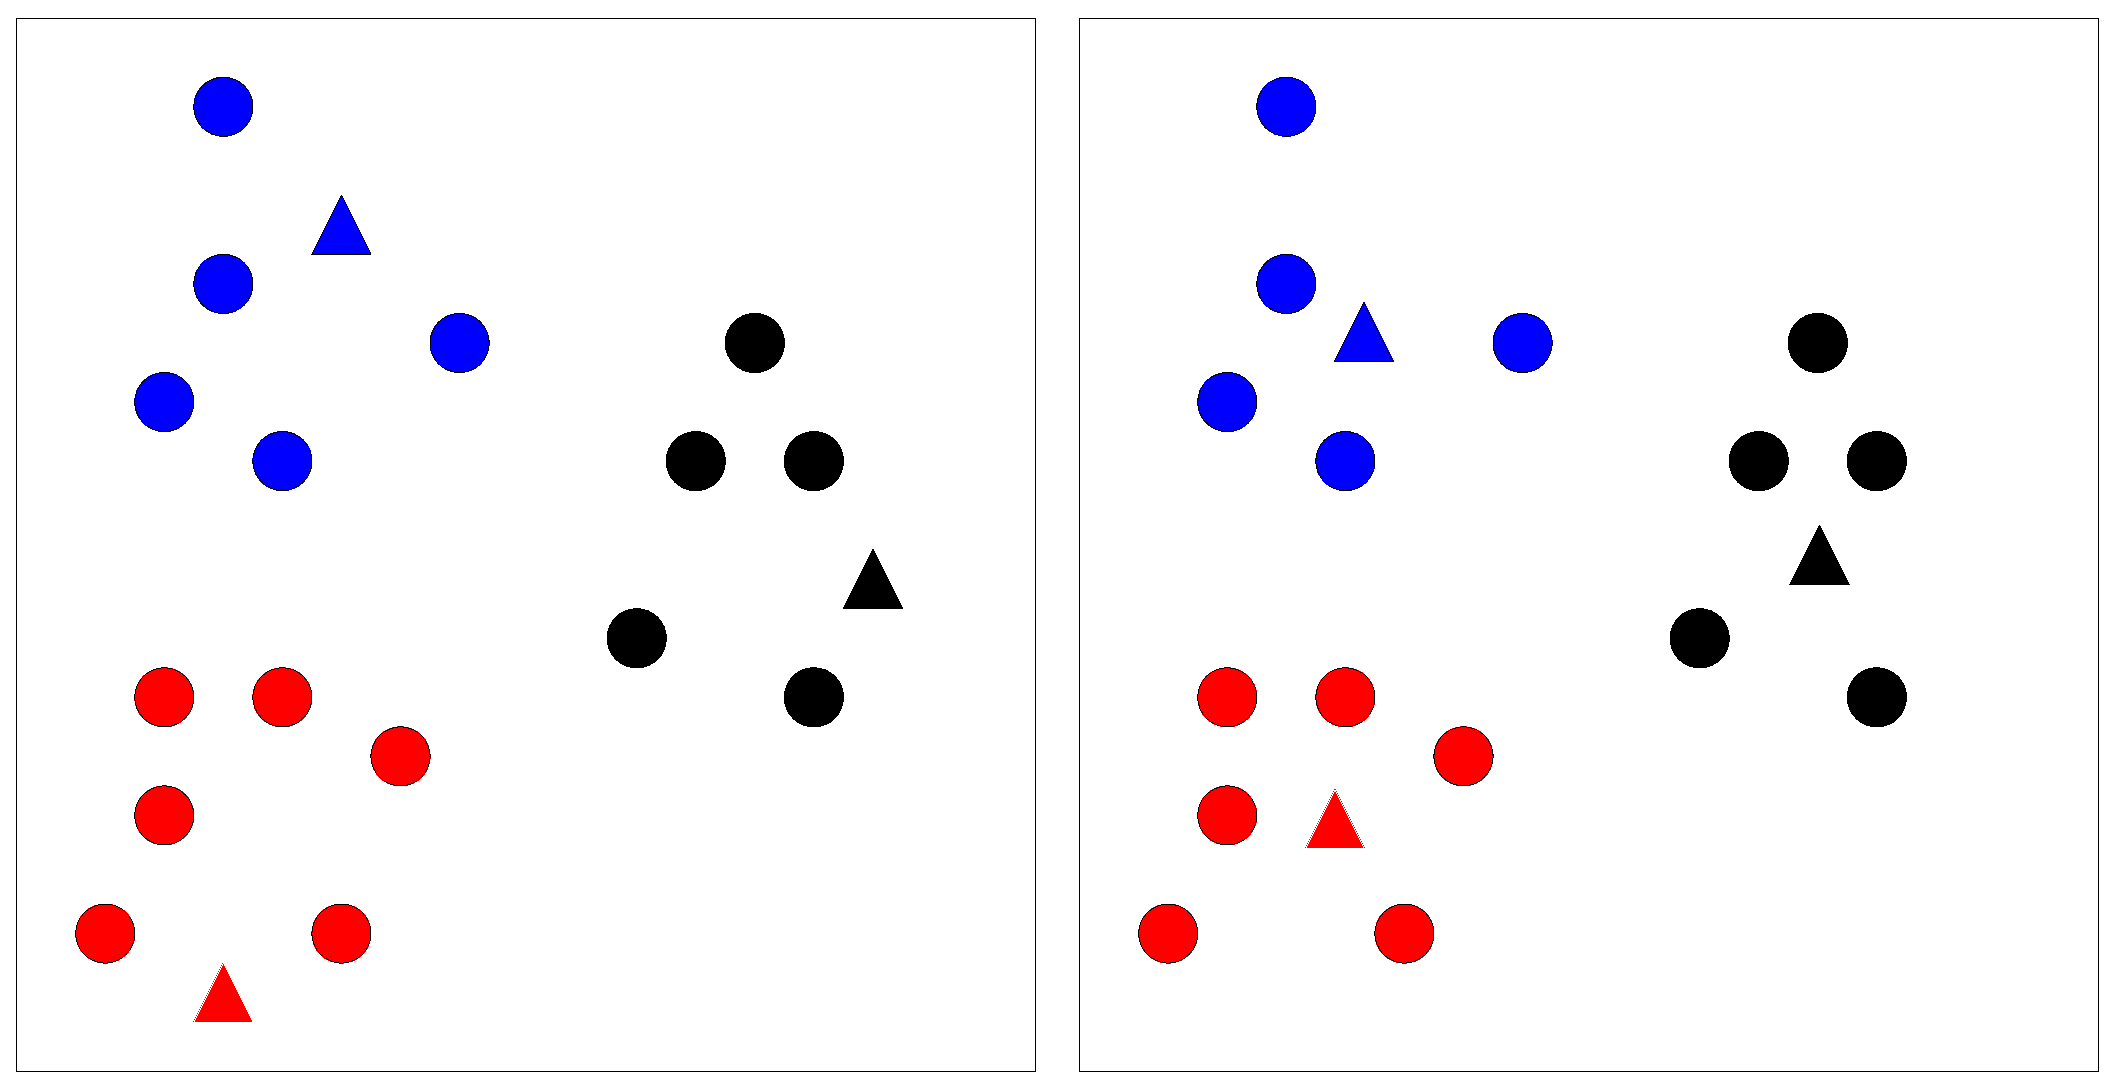
\includegraphics[scale=0.3]{\rootpath/worksheets/performance_test/figures/kmeans}
\caption{On the left data points are assigned to the nearest centroid (cluster) based on the calculated distances. On the right, a new centroid is computed for each cluster.}\label{fig:kmeans}
\end{figure}

The implementations follows a template similar to that of Map-Reduce\cite{dean2008mapreduce}, known from functional programming, as well as the Google and Hadoop MapReduce frameworks. MapReduce employs a set of mappers to apply a function to each data point. This function outputs a number of results, that are then aggregated to the final result using a reducer. Our $k$-means MapReduce process is illustrated in \bsref{fig:kmeans_mapreduce}. A set of mappers is assigned a set of vectors, for which it calculates the distance to each of the $k$ cluster centroids and assigns it to the nearest cluster. A reducer will then aggregate the results from the mappers and calculate the new cluster centroids. The process will continue until the stated number of iterations are achieved.

\begin{figure}
\centering
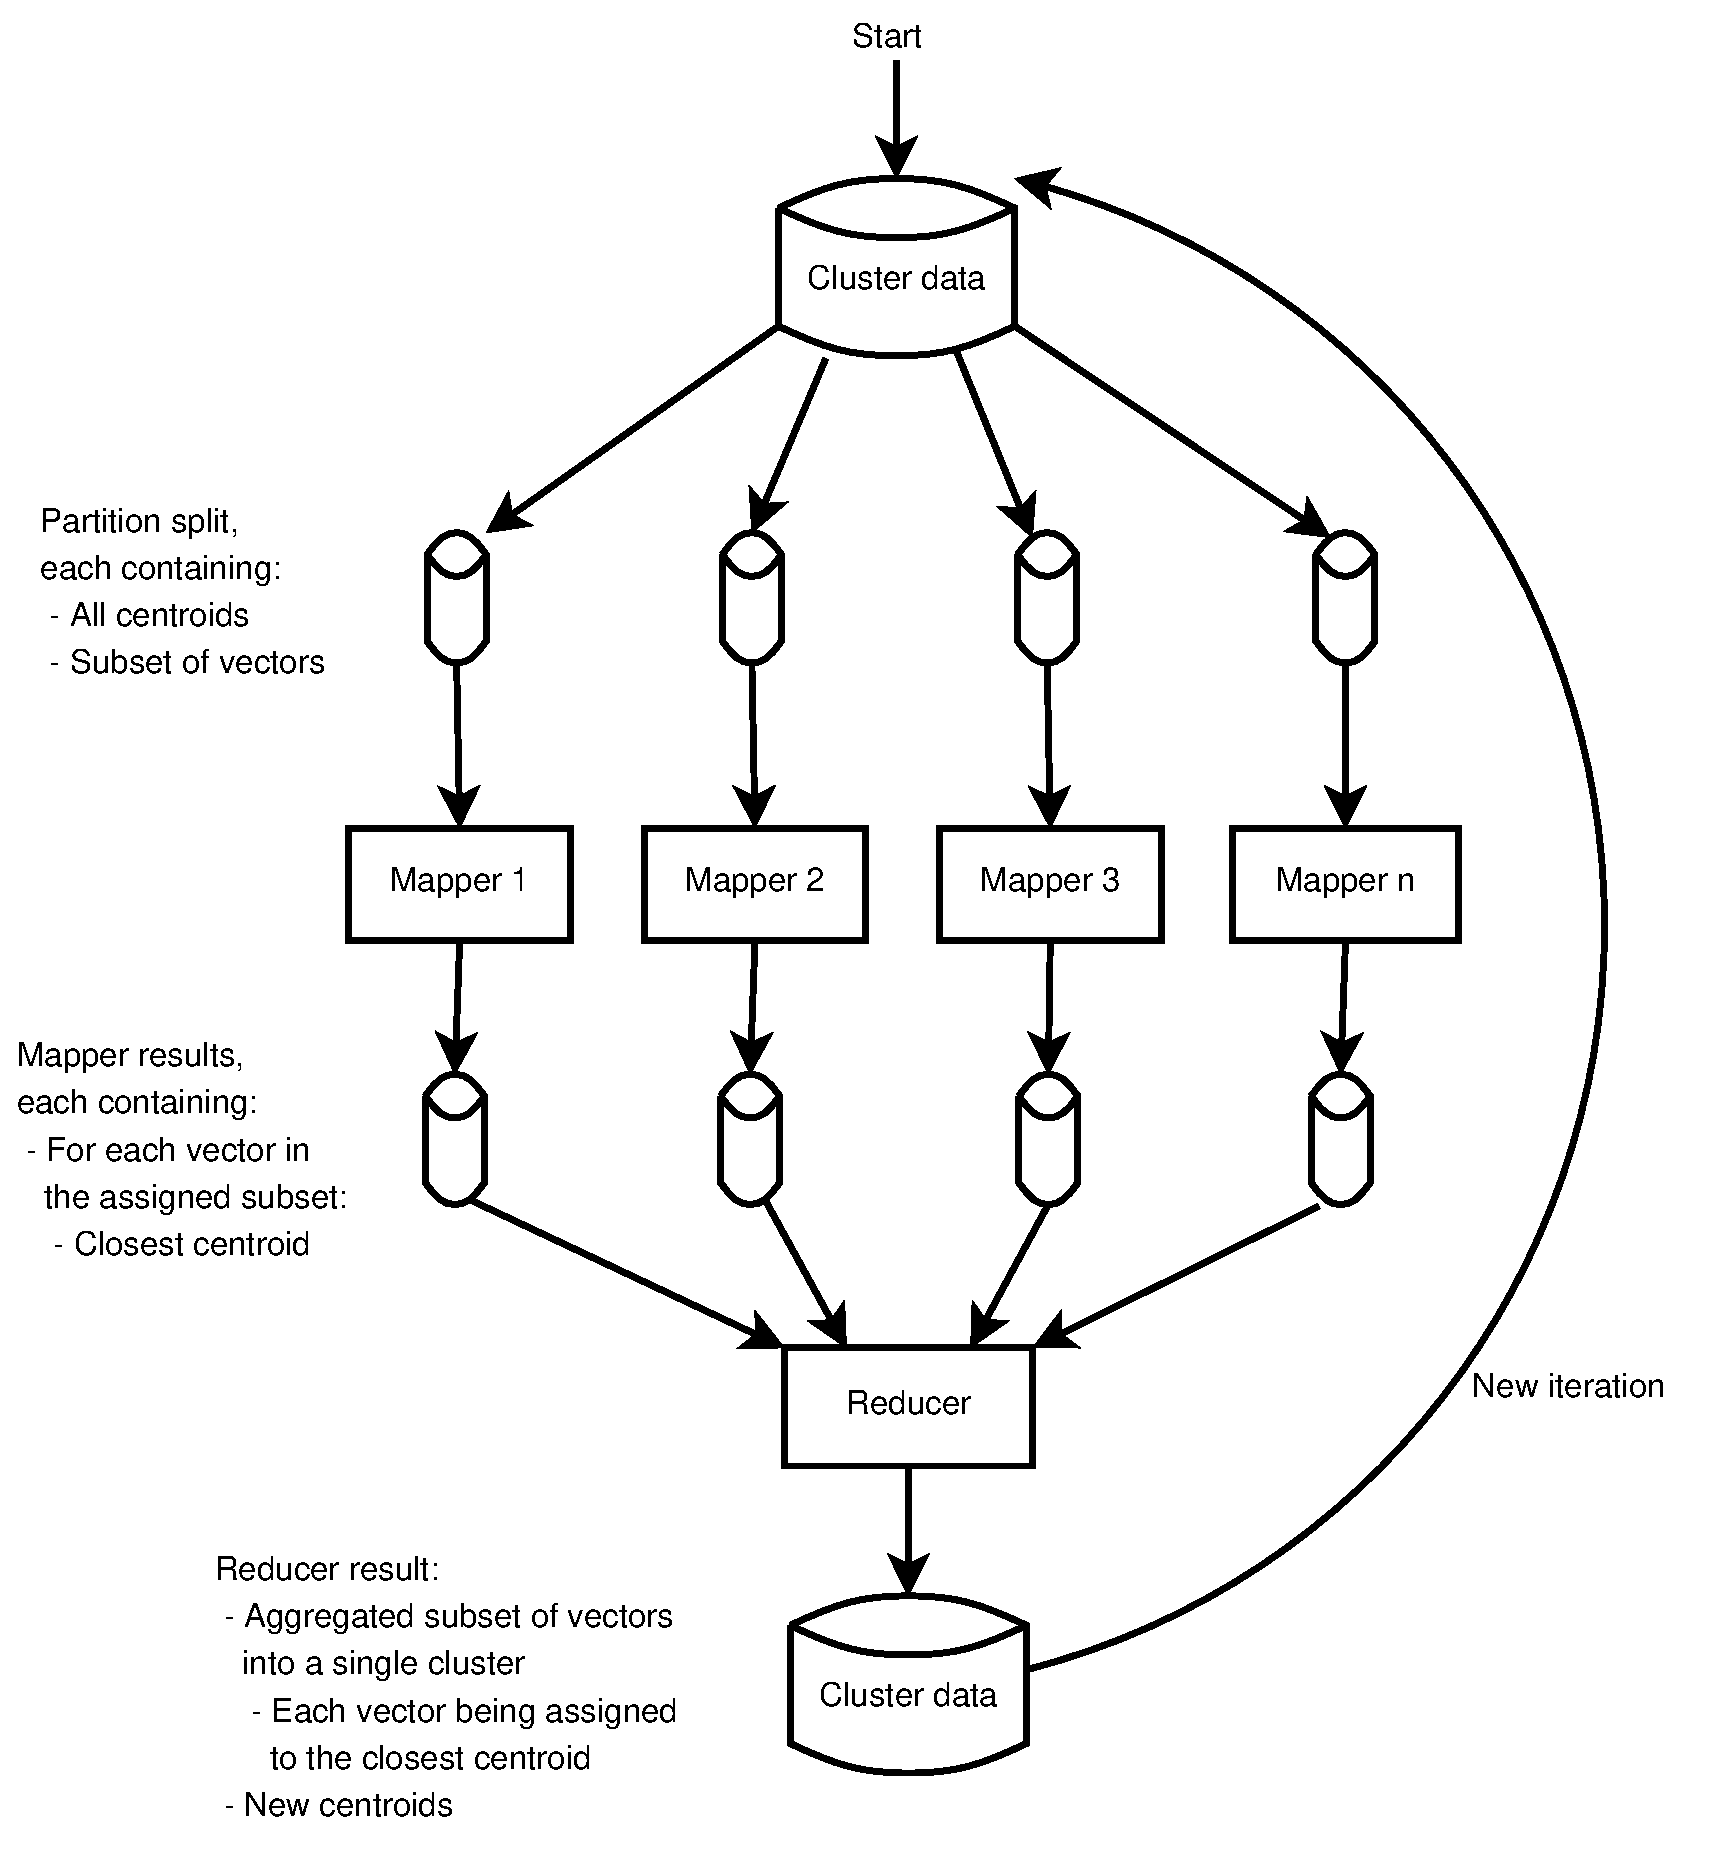
\includegraphics[scale=0.5]{\rootpath/worksheets/performance_test/figures/mapreduce_figure}
\caption{$k$-means MapReduce process}\label{fig:kmeans_mapreduce}
\end{figure}



\subsection{Test Design}
In order to design the needed test cases, an initial test run was done. A description of the initial test run as well as its results can be viewed in \bsbilagref{app:explo_result}. The test run showed little difference between the selected concurrency models and revealed a need for both stressing the synchronization mechanisms of the selected concurrency models as well as scaling the size of the workload. Therefore it was decided to investigate both how the concurrency models affect high workload tasks and high synchronization tasks. To this end, two test cases were designed. Both test cases are based on a data set of 100 integer data point vectors. The first test investigates how the selected concurrency models affect a task with a high degree of concurrent work but a low degree of synchronization. The second investigates how the selected concurrency models affects a task with a low degree of concurrent work and a high degree of synchronization. In order to mitigate potential outlying results, each test were run five times and the mean runtime is used as the result. In the context of performance analysis, only the effort taken to cluster the data is of interest, as opposed to the resulting clustering. Due to this, randomly generated data is sufficient.

\kasper[inline]{Description of how tests where created based on previous test run}

\subsection{Work Intensive Tests}
The work intensive tests consists of the two tests: test $A$ and test $B$. The parameters for the tests are shown in \bsref{tab:test_description_work_intensive}. These tests are designed to investigate the impact of the selected concurrency models on workload with a low degree of synchronization and a large amount of concurrent work. The only thing that differs in the implementations is the concurrency mechanisms, and combined with the low degree of synchronization, we expect that the performance of the concurrency models will be close to similar.

Test $A$ is based on a fixed size data set, while the number of mapper tasks will be scaled up. The goal is to determine how the selected concurrency models scale as more concurrent tasks are added. Five clusters are created, using 1 to 10 mapper tasks. The algorithm will run for 100 iterations\andreas{How do we get to these numbers?}. The amount of mappers, has been chosen with consideration to the amount of physical and logical cores in hardware used for the test, described further in \bsref{subsec:hardware}. Our implementations uses one thread to coordinate and drive the calculations, as well as running the reducer. Consequently, making 3 mapper tasks will utilize 4 cores concurrently.

Test $B$ is based on a fixed number of concurrent mapper tasks as well as a fixed number of iterations, while the size of the dataset will be scaled up. Scaling up the size of the dataset will increase the workload that is run concurrently. The goal of the test is to investigate how the selected concurrency models affects a task with a high concurrent workload. The test will employ a dataset of 1,000,000 to 5,000,000 vectors along with seven mapper tasks. The test will run for 100 iterations. We expect to see a decreasing difference in performance as the vector size increases, since an increasing amount of time will be spend on clustering and little time spent on synchronization, due to the fixed low amount of iterations.\toby{Evt. slet den her sætning fordi vi har allerede fortalt om det i starten af denne sketion - ellers skal der være en lignende expectation til test A}

\begin{center}
\begin{table}[h]
\centering
\begin{tabular}{c|cccc}
       & \# Vectors        & \# Mappers			 	& \# Clusters & \# Iterations \\ \hline
Test $A$ & 2,000,000            & 1-10        			& 5           & 100      \\
Test $B$ & 1,000,000-5,000,000  & 7          			& 5           & 100
\end{tabular}
\end{table}
\captionof{table}{Test descriptions for work intensive tests} \label{tab:test_description_work_intensive} 
\end{center}

\subsubsection{Distance Measure}
A large part of the computations involved in the $k$-means algorithm, lies in calculating the distance between each of the data points and the cluster centroids. Different ways of calculating this distance exist. Simple, yet efficient, calculations such as Manhattan and Euclidean\cite[p. 41]{amatriain2011data} distances are fast to compute, where as the more complex similarity measures such as Pearson Correlation Coefficient and Cosine similarity\cite[p. 42]{amatriain2011data}\cite{breese1998empirical} are slower to compute but provide a more accurate result.

For the work intensive tests the \ac{PCC} will be used, as it represents one of the most complex computations. Having a complex distance calculation will increase the workload that will be run concurrently. The \ac{PCC} is defined as\cite[p. 4]{breese1998empirical}:
\begin{equation}\label{pearsonverbose}
\frac{cov(a,i)}{\sigma_a \times \sigma_i} = \frac{\sum_j(v_{a,j}-\bar{v}_a)(v_{i,j}-\bar{v}_i)}{\sqrt{{\sum_j}(v_{a,j}-\bar{v}_a)^2 \sum_j(v_{i,j}-\bar{v}_i)^2}}
\end{equation}

where $cov(a,i)$ is the covariance between the two vectors $a$ and $i$ and $\sigma_a \times \sigma_i$ is the product of the vectors standard deviations.

\subsection{Synchronization Intensive Tests}
The synchronization intensive test will consist of the two tests: test $C$ and test $D$. The parameters for the tests are shown in \bsref{tab:test_description}. These tests are designed to investigate how the selected concurrency models affect a concurrent computation with a high degree of synchronization. 

Test $C$ is based on a fixed size data set, while the number of mapper tasks will be scaled up.  The test will be based on a data set of 10.000 vectors. Five clusters are created, using 1 to 10 mapper tasks. The algorithm will run for 100.000 iterations. As with the previous tests, the amount of mappers have been chosen based on the underlying hardware. We expect a decreasing run time while scaling up to 7 mappers, as that will equal into 8 cores running concurrently. However, the biggest decrease should be seen up to 3 mappers, as the physical cores are known to perform vastly better than hyperthreaded cores\andreas{Need reference}. After 7 mappers, we expect the run time to be slower, as coordination between the threads causes overhead in the computation.

Test $D$ is based on a fixed number of concurrent tasks as well as a fixed size dataset, while the number of iterations will be scaled up. Synchronization is applied whenever mappers delegate their work to the reducer. Scaling up the number of iterations will increase the number of times synchronization is executed for each of the selected models. As such this test seeks to investigate the impact each of the selected concurrency model has on the performance of the clustering algorithm\andreas{Fortæller den sætning noget?}. It is our expectation that each model will have fairly close performance overhead\andreas{Synchronization overhead?}, but due to different reasons. 
\andreas[inline]{It is our expectation that the different synchronization overhead will be clear in this test, and an increasing difference will be seen as the number of iterations increase and thereby the amount of synchronization.}
The test will employ a dataset of 10,000 vectors along with seven mapper tasks. The number of iterations will be scaled from 10,000 to 100,000 in intervals of 10,000. The amount of mappers was chosen to be 7, since it will enable all 8 logical cores to work concurrently.

The parameters of the two tests are depicted in \bsref{tab:test_description}.

\begin{center}
\begin{table}[h]
\centering
\begin{tabular}{c|cccc}
       & \# Vectors        & \# Mappers			 	& \# Clusters & \# Iterations \\ \hline
Test $C$ & 10,000            & 1-10        			& 5           & 100,000      \\
Test $D$ & 10,000			 & 7          			& 5           & 10,000-100,000
\end{tabular}
\end{table}
\captionof{table}{Test descriptions for synchronization intensive tests} \label{tab:test_description} 
\end{center}

\subsubsection{Distance Measure}
The Manhattan distance will be used for the synchronization intensive tests as it represents a simple distance calculation. Having a simple calculation will limit the amount of work spent on computing the clusters. As such the work done by the concurrency models will have a greater impact on the results. The Manhattan distance is defined as\cite[p. 41]{amatriain2011data}:
 
\begin{equation}\label{eq:mandistance}
man(v_a,v_i)=\sum_{j=1}^{n}\lvert v_{a,j}-v_{i,j}\rvert
\end{equation}

where $man(v_a,v_i)$ is the Manhattan distance between the two vectors $v_a$ and $v_i$ and $n$ is the length of these vectors. $v_{a,j}$ and $v_{i,j}$ are the $j$'th item of the vectors $v_a$ and $v_i$ respectively.

\subsection{Test Setup}\label{subsec:hardware}
Listing the specification of the hardware is mainly due to reproducibility and transparency. The tests will be performed on a high-grade consumer PC, specifically a Macbook Pro from 2014, with the following specifications:
\begin{itemize}
	\item \textbf{CPU} Quad Core 2.8 GHz Intel Core i7 \footnote{\url{http://ark.intel.com/products/83503/Intel-Core-i7-4980HQ-Processor-6M-Cache-up-to-4_00-GHz}}
	\item \textbf{Memory} 16 GB 1600 MHz DDR3L
	\item \textbf{\ac{OS}} OSX 10.10.1 (14B25)
	\item \textbf{\ac{JVM}} Java HotSpot(TM) 64-Bit Server VM (build 25.20-b23, mixed mode)
\end{itemize}
%The result of the performance test is only interesting when comparing the different implementations

The most noticeable specification of the test setup is the amount of cores on the \ac{CPU}. There are 8 logical cores, where 4 of them are physical. The amount of cores will enable us to test the scalability of the different implementations. In some research\cite{harris2003language}, the scalability of different implementations varied after surpassing 35 cores. It could be interesting to employ our test in such a setting.

The test will be done with the Wi-Fi turned off and all applications closed but the test application. This is done to eliminate other programs hogging resources during the test run. The machine will be plugged into a power outlet the entire time to enable maximum clocking of the \ac{CPU}.

\section{Test Implementations}
This section presents a small overview of the implementations used in the performance test. As described in \bsref{sec:intro_scope}, one implementation has been made for each of the selected concurrency models, and all of the chosen languages run on the \ac{JVM}. The \ac{TL} based implementation is done in Java, the \ac{STM} based implementation in Clojure and the actor based implementation in Scala. The calculations needed to cluster vectors is implemented in Java and reused throughout all implementations. This ensures that the computations themselves do not impact the results. Each implementation simply creates its own skeleton for driving the clustering process using its corresponding concurrency model, and employs the common clustering implementation to handle the clustering details. 

In order to provide a fair comparison between the implementations execution time, the amount of work they do must be equivalent. As the implementations share the same code base for cluster calculations, it is only the concurrency mechanism and driving skeleton which impacts the results. To verify this, we have made a static set of vectors, which we can run across all the implementations, and compare the result of the final means. Running over this test data all implementations produce the the same clustering. While this is not a formal verification, is does provide a positive indication that the same work is performed across the implementations.\toby{Se hvad Lone sagde til den originale sætning der var her og om det her er bedre.}
\andreas[inline]{The source code is available at the enclosed DVD together with instructions for running it}

\subsection{\ac{TL} Implementation}
Java has been chosen for the \ac{TL} based implementation because of its well documented support for the concurrency model and its widespread use. The \ac{TL} implementation maps the reducer and mappers directly to their own thread by providing an implementation of the \bscode{Runnable} interface. A producer consumer setup, controlled by a semaphore, is employed. The mappers cluster the subset of data which they receive and pass the result to the reducer by adding it to a queue. Finally the reducer is signalled via the semaphore.\andreas{Who is the producer/consumer?} The reducer aggregate the results as they become available from the mappers  and prepares for the next iteration by calculating the new cluster means. The \bscode{run} method of the \bscode{Mapper} class is shown in \bsref{lst:tl_implementation}. On line 3 the mapper uses the common clustering service to cluster the data it received according to the supplied means. The resulting clustering is added to a queue shared with the reducer and all other mappers on line 6. Access to the queue is synchronized by using a lock, preventing other mappers, as well as the reducer from accessing the queue while the mapper adds the result. Finally the mapper signals the reducer using the semaphore on line 8. All non local variables, such as the data and queue, are supplied in the \bscode{Mapper} classes constructor.

\begin{lstlisting}[float,label=lst:tl_implementation,
  caption={\ac{TL} Implementation},
  language=Java,  
  showspaces=false,
  showtabs=false,
  breaklines=true,
  showstringspaces=false,
  breakatwhitespace=true,
  commentstyle=\color{greencomments},
  keywordstyle=\color{bluekeywords},
  stringstyle=\color{redstrings}]  % Start your code-block

    @Override
    public void run() {
        Clustering clustering = ClusteringService.ClusterKMeansMSIncremental(data, means);
        //Hand off data
        lock.lock();
        queue.add(clustering);
        lock.unlock();
        semaphore.release(1);
    }  
\end{lstlisting}

\subsection{\ac{STM} Implementation}
As our preliminary investigation showed in \bsref{sec:prelim_stm}, a number of programming languages and libraries to support \ac{STM} have emerged. To our knowledge, Clojure is the only official language running on the \ac{JVM} that natively support \ac{STM}. The native support enables compiler and runtime optimisations, which potentially is a big performance factor. Due to these reasons, Clojure has been chosen as the language for the \ac{STM} implementation.

\toby[i]{Måske nævn også at der ikke er noget shared state generelt - kun kun med specielle constructs i sproget der bruges i transations. Så en udvikler kan ikke pille i state udenom, som man kan i andre sprog - se evt. side 301 i JVM mastering syncrhonization bogen. Revidering: Der bliver snakket om dette længere nede, måske bare nævn det som en grund til valg af sprog og refer ned?}

\subsubsection{Clojures \acs{STM} Design}
In \bsref{subsec:stm:variations_in_design} we discussed the impact of \ac{STM} design variations. In the following section, we will briefly describe the \ac{STM} design in Clojure.

The isolation level of transactions in Clojure is strong. Clojure employs a special type for references named \bscode{ref}\footnote{\url{http://clojuredocs.org/clojure.core/ref}}. It is only possible to modify this reference  inside transactions. Due to this, Clojure does not have to account for modifications of references happening outside of transactions, and can secure strong isolation without any performance penalty. This is a property made possible due to transactions being built into the language. 

It is the programmers responsibility not to do any irreversible actions, such as \ac{IO}, in a transaction. Clojure supplies a macro, \bscode{!io}, which raises a runtime exception if a marked function is called in a transaction. If an exception is raised inside a transaction, the transaction is aborted and the exception is propagated out of the transaction\footnote{\url{http://clojuredocs.org/clojure.core/dosync}}. As discussed in \bsref{subsec:stm:side_effects}, this does not change the way the programmer should handle exceptions compared to sequential code. 

It is however not possible to wrap a transactional block around an existing implementation, to secure it runs correct concurrently. This is due to the special \bscode{ref} construct in Clojure, that must be used to enable atomicity in a transaction. The composability of \ac{STM} and the other language constructs in Clojure is limited by design. It is only possible to modify the aforementioned special types in a transaction. Other types in Clojure cannot leverage transactions to synchronize, but this is part of the design, as they are immutable. 

It is possible to nest transactions in Clojure, however the inner transaction will first commit when the outer transaction does.

Conditional synchronization is not directly supported in Clojure, as the \bscode{dosync} function does not take any conditional variables and the language does not have a \bscode{retry} construct. As such conditional synchronization must be achieved by other means, such as busy waiting.

Reads in Clojure are invisible\cite{nielsen2010benchmarking}, which means that when a transaction reads, it does not communicate its operations to other transactions. Instead metadata is used to validate each transaction. To manage contention, Clojure uses a strategy called Priority\cite{nielsen2010benchmarking}. This strategy allows older transactions, in respect to alive time, to run in favour of younger transactions. Research\cite{nielsen2010benchmarking} has shown that in most cases this is a competitive strategy compared to other contention strategies. 

\subsubsection{Clojure Implementation}
\begin{lstlisting}[float,label=lst:stm_implementation,
  caption={\ac{STM} Implementation},
  language=clojure,  
  showspaces=false,
  showtabs=false,
  breaklines=true,
  showstringspaces=false,
  breakatwhitespace=true,
  commentstyle=\color{greencomments},
  keywordstyle=\color{bluekeywords},
  stringstyle=\color{redstrings}]  % Start your code-block
  
  (def clusters (ref '()))
    
  (defn mapper [data means clusters]
    (let [cluster (clustering data means)]
      (dosync
        (commute clusters conj cluster)))
    clusters)
\end{lstlisting}

The central point of the implementation, is shown at line 1 in \bsref{lst:stm_implementation}. It shows a reference to at list, named \bscode{clusters}. When calculating the centroids, a vector containing the initial values, is split up into the amount of mappers defined. The mappers work on each of their slice, and add their result to the \bscode{clusters} list. The reducer then reduces the list, by merging the results and calculating the centroids.

Line 3 in \bsref{lst:stm_implementation} shows the definition of the mapper function. Each mapper is executed in a \bscode{future}\footnote{\url{http://clojuredocs.org/clojure.core/future}}, which is a concurrency unit, that yields a non-blocking result. The future can be queried for the result, on which it will block until the result is available. On line 4 is the actual calculation which is bound to a value named \bscode{cluster}. The \bscode{cluster} value is then added into the list of \bscode{clusters} on line 6, by using the \bscode{commute}\footnote{\url{http://clojuredocs.org/clojure.core/commute}} function. \bscode{commute} is a special function in Clojure, that can be used to update references inside transactions, when the update is commutative. That is, the order the list is updated in, does not matter. For non-commutative operations, \bscode{alter}\footnote{\url{http://clojuredocs.org/clojure.core/alter}} can be used, albeit it is not as fast as \bscode{commute}.\andreas{Need cite! Noget med, at alter genlæser ved read, gør commute ikke}\toby{Yes ville være lækkert :)} All this happens inside the \bscode{dosync} transaction block, that ensures synchronisation in concurrent operations. The reducer must wait until all the mappers have updated the list with their result.\toby{Why?} This is enforced by dereferencing the futures, that the mappers are executed in, which will force synchronisation, so the reducer receives all the intermediate clustering results.

\subsection{Actor Implementation}
The Scala language has been selected for the actor based implementation, as it has good support for actors in the form of the Akka actor framework. Akka is a well-known and popular actor implementation\toby{kan cite "efficient testing artikeln" om at det er en popular actor implementation hvis det er} used by companies such as Cisco, Ebay, Amazon and Blizzard.\footnote{\url{http://akka.io/}} Akka has even replaced the Scala Actors as the default actor framework for Scala applications\footnote{Changes in Ver. 2.10.0: \url{http://www.scala-lang.org/download/changelog.html}}.

\subsubsection{Akka Adherence to Semantic Properties}\toby{Evt. hav det efter implementation bliver forklaret hvis det passer bedre}
The Akka framework uses light-weight actors which means that several actors may share a single thread\cite[p. 13]{akkaDoc}, as discussed in \bsref{ssec:abstraction_over_threads}. 
In relation to the semantic properties of the actor model, mentioned in \bsref{ssec:actor_s_properties}, Akka adheres to the property of atomic processing of messages and location transparency. Location transparency is ensured by using actor references, that are created by specifying a name together with an actor type\cite[p. 24]{akkaDoc}. 

However, the properties of fairness and encapsulation are not adhered to, in order to improve performance. Akka employs an at-most-once message delivery semantics which means that a message is either delivered zero or one times, as that has the lowest implementation overhead\cite[p. 27]{akkaDoc}. This violates the fairness property which assumes that all messages are eventually delivered. However, it is possible to enforce stricter reliability in Akka, but at the cost of local-only deployment\cite[p. 29]{akkaDoc}. Akka does also not adhere to the encapsulation property, as it implements message passing by sending message contents by reference which enables the possibility of shared mutable state, as discussed in \bsnameref{sssec:safe_msg_passing}. However this only applies to local actors, when messages are sent to remote actors the message contents are copied instead. Additionally, these are the default serialization settings and Akka enables the programmer to specify different serialization techniques\cite[p. 219]{akkaDoc}.

As Akka does not adhere to all the semantic properties of the actor model, it introduce risks that the conceptual actor model avoids by design, e.g. deadlocks. To alleviate these issues Akka has some actor best practices, that the programmer should adhere to. E.g. do not pass mutable objects between actors\cite[p. 12]{akkaDoc}. It is a trade-off between programmer concerns and implementation performance.

%MERE:
%Akka facilitates fault toleracne, persistence and automatic load balancing.
	% se side 1-2 i Akka scala documentation
	% og se efficient testing artikeln s. 12 (under actors)

%Quote fra efficient testing artikeln:
%Note that exploiting the benefits of the actor model for programming does not require a language that enforces strict actor semantics; it is sufficient to have a library providing asynchronous messaging between concurrent objects, and to adhere to coding conventions for avoiding shared state.
\subsubsection{Akka Implementation}
A central \bscode{Master} actor is responsible for driving the clustering process. It handles distribution of data to the mappers and running the clustering process for the required number of iterations. \bsref{lst:actor_implementation} shows the \bscode{Mapper} and \bscode{Reducer} actors of the implementation. On line 3-7 the behaviour method scope is defined for the \bscode{Mapper} actor. There is only a single behaviour method defined for this actor, which is for a \bscode{MapWork} message on line 4. Such a message contains the data that should be clustered, the cluster centroids and a reference to the \bscode{Reducer} actor, sent from the \bscode{Master} actor. On line 5 the \bscode{Mapper} clusters its data segment using the common clustering service, followed on line 6 by sending the result as a \bscode{MapperResult} message to the \bscode{Reducer}.

On line 10-24 the \bscode{Reducer} actor is defined. First on line 11-12 some isolated state variables are defined, followed by the behaviour method scope on line 14-24.
The \bscode{Reducer} actor receives the result from \bscode{Mappers} on line 15, where the \bscode{Reducer} merges the received intermediate result with the previously received results. On line 19-22, if the current message is the last message then the \bscode{Reducer} calculates the means for the new clusters and sends the \bscode{ReducerResult} message to the master actor.

\begin{lstlisting}[float,label=lst:actor_implementation,
  caption={Actor Implementation},
  language=Scala,  
  showspaces=false,
  showtabs=false,
  breaklines=true,
  showstringspaces=false,
  breakatwhitespace=true,
  commentstyle=\color{greencomments},
  keywordstyle=\color{bluekeywords},
  stringstyle=\color{redstrings}]  % Start your code-block

  class Mapper extends Actor {

    def receive = {
      case MapWork(data: List[Vector], means: List[Vector], reducer: ActorRef) =>
        val clustering: Clustering = ClusteringService.ClusterKMeansMSIncremental(data, means)
        reducer ! MapperResult(clustering)
    }
  }

  class Reducer(nrActors: Int, nrClusters: Int) extends Actor {
    var consumedMessages: Int = 0
    var clustering: Clustering = new Clustering(nrClusters)

    def receive = {
      case MapperResult(c: Clustering) =>
        clustering.mergeWith(c);
        consumedMessages += 1

        if (nrActors == consumedMessages) {
            clustering.calcMeansUsingMeanSum();
            context.parent ! ReducerResult(clustering)
        }
    }
  }  
\end{lstlisting}


\section{Test Results}

\subsection{Work Intensive Tests}
\kasper[inline]{Akka passes by reference = faster, especially with fast data}

\begin{center}
\begin{table}[h]
\centering
\begin{tabular}{l|cll|cll}
             & \multicolumn{3}{c|}{Milliseconds} & \multicolumn{3}{c}{Normalized} \\
Vectors & TL     & STM     & Actor     & TL      & STM      & Actor     \\ \hline
1.000.000                   &     68572       &      68806       &    68541  &	 1,00   & 1,00 &    1,00    \\
2.000.000                   &     137677      &      138041      &    137249  &  1,00   & 1,01 &    1,00    \\
3.000.000                   &     206000      &      206559      &    205472  &  1,00   & 1,01 &    1,00    \\
4.000.000                   &     274622      &      275882      &    273920  &  1,00   & 1,01 &    1,00    \\
5.000.000                   &     344108      &      344939      &    343521  &  1,00   & 1,00 &    1,00    \\
6.000.000                   &     456160      &      467615      &    453272  &  1,01   & 1,03 &    1,00    \\
7.000.000                   &     658594      &      658302      &    625962  &  1,05   & 1,05 &    1,00    \\
\end{tabular}
\captionof{table}{Test $B$ results. Scaling the amount of vectors}\label{table:test_results_concurrent_tasks}
\end{table}
\end{center}

\begin{figure}[h]
\centering
\begin{tikzpicture}[scale=1.2]
	\begin{axis}[
		legend entries={\acs{TL},\acs{STM}, Actor},
		legend pos=north west,
		grid = both,
		xlabel=Vectors,
		ylabel=Miliseconds,
		xmin=0,
		ymin=0, 
		label=fig:tr_scale_iterations]		
	\addplot[color=red,mark=x] coordinates {
%		(1,21)
		(100000,68572)
		(200000,137677)
		(300000,206000)
		(400000,274622)
		(500000,344108)
		(600000,456160)
		(700000,658594)
	};
	\addplot[color=blue,mark=x] coordinates {
%		(1,33)
		(100000,68806)
		(200000,138041)
		(300000,206559)
		(400000,275882)
		(500000,344939)
		(600000,467615)
		(700000,658302)
	};
	\addplot[color=green,mark=x] coordinates {
%		(1,			27)
		(100000,68541)
		(200000,137249)
		(300000,205472)
		(400000,273920)
		(500000,343521)
		(600000,453272)
		(700000,625962)
	};
	\end{axis}
\end{tikzpicture}
%\captionsetup{justification=centerlast, margin=10ex, labelfont=bf, textfont=it, format=plain, labelformat=default, labelsep=endash, font=small}
\caption{Test $B$. Visual representation of results for scaling number of vectors}\label{fig:test_results_iterations}
\end{figure}

\begin{figure}[h]
\centering
%0 - aramente   1 - Às vezes   2 - Quase sempre   4 - Sempre
\pgfplotstableread{
  %TL    	%STM  	%Actor
0 1.00	1.01	1.00
1 1.00	1.01	1.00
2 1.01	1.03	1.00
3 1.05	1.05	1.00
4 1.01	1.02	1.00
}\dataset
\begin{tikzpicture}
\begin{axis}[ybar,
%        width=12cm,
		width=\textwidth,
        height=8cm,
        ymin=0.8,
        ymax=1.2,        
        ylabel={Value-normalized runtime},
        xlabel={Iterations},
        xtick=data,
        xticklabels = {
            \strut 2\,000\,000,
            \strut 4\,000\,000,
            \strut 6\,000\,000,
            \strut 7\,000\,000,
            \strut average
            %Category 5,
            %Category 6
        },
        %xticklabel style={yshift=-10ex},
        major x tick style = {opacity=0},
        minor x tick num = 1,
        minor tick length=2ex,
        every node near coord/.append style={
                anchor=west,
                rotate=90
        },
        legend entries={\ac{TL} ,\ac{STM} ,Actor },
        legend columns=3,
        legend style={draw=none,nodes={inner sep=3pt}},
        ]
\addplot[draw=black,fill=red, nodes near coords] table[x index=0,y index=1] \dataset; %TL
\addplot[draw=black,fill=blue, nodes near coords] table[x index=0,y index=2] \dataset; %STM
\addplot[draw=black,fill=green, nodes near coords] table[x index=0,y index=3] \dataset; %Actor
\end{axis}
\end{tikzpicture}
%\captionsetup{justification=centerlast, margin=10ex, labelfont=bf, textfont=it, format=plain, labelformat=default, labelsep=endash, font=small}
\caption{Test $B$. Value-normalized results for scaling number of vectors}\label{fig:value_norm_test2}
\end{figure}


\subsection{Synchronization Intensive Tests}
\begin{center}
\begin{table}[h]
\centering
\begin{tabular}{l|cll|cll}
             & \multicolumn{3}{c|}{Milliseconds} & \multicolumn{3}{c}{Normalized} \\
Mapper Tasks & TL     & STM     & Actor     & TL      & STM      & Actor     \\ \hline
1                   &     498792      &      510154      &    513734  &	 1.00   & 1.02 &    1.03    \\
2                   &     263507      &      272869      &    268115  &  1.00   & 1.04 &    1.02    \\
3                   &     186577      &      194757      &    191510  &  1.00   & 1.04 &    1.03    \\
4                   &     159645      &      173548      &    161304  &  1.00   & 1.09 &    1.01    \\
5                   &     171512      &      176791      &    173379  &  1.00   & 1.03 &    1.01    \\
6                   &     154108      &      163118      &    161729  &  1.00   & 1.06 &    1.05    \\
7                   &     152569      &      158746      &    163118  &  1.00   & 1.04 &    1.07    \\
8                   &     154261      &      168380      &    162539  &  1.00   & 1.09 &    1.05    \\
9                   &     171477      &      188020      &    188653  &  1.00   & 1.10 &    1.10    \\
10                 &     163490      &      182868      &    179347  &	 1.00   & 1.12 &    1.10    \\
\end{tabular}
\captionof{table}{Test $C$ results. Scaling number of mapper tasks}\label{table:test_results_concurrent_tasks}
\end{table}
\end{center}

\begin{figure}[h]
\centering
\begin{tikzpicture}[scale=1.2]
	\begin{axis}[
		legend entries={\acs{TL},\acs{STM}, Actor},
		legend pos=north east,
		grid = both,
		xlabel=Mapper tasks,
		ylabel=Miliseconds,
		xmin=0,
		ymin=0, 
		label=fig:tr_scale_mappers]		
	\addplot[color=red,mark=x] coordinates {
		(1,498792)
		(2,263507)
		(3,186577)
		(4,159645)
		(5,171512)
		(6,154108)
		(7,152569)
		(8,154261)
		(9,171477)
		(10,163490)
	};
	\addplot[color=blue,mark=x] coordinates {
		(1,510154)
		(2,272869)
		(3,194757)
		(4,173548)
		(5,176791)
		(6,163118)
		(7,158746)
		(8,168380)
		(9,188020)
		(10,182868)
	};
	\addplot[color=green,mark=x] coordinates {
		(1,513734)
		(2,268115)
		(3,191510)
		(4,161304)
		(5,173379)
		(6,161729)
		(7,163118)
		(8,162539)
		(9,188653)
		(10,179347)
	};
	\end{axis}
\end{tikzpicture}
%\captionsetup{justification=centerlast, margin=10ex, labelfont=bf, textfont=it, format=plain, labelformat=default, labelsep=endash, font=small}
\caption{Test $C$ results. Visual representation of results for scaling number of mapper tasks}\label{fig:test_results_concurrent_tasks}
\end{figure}

\begin{figure}[h]
\centering
%0 - aramente   1 - Às vezes   2 - Quase sempre   4 - Sempre
\pgfplotstableread{
  %TL    	%STM  	%Actor
0	1		1.02		1.03
1	1		1.04		1.02
2	1		1.04		1.03
3	1		1.09		1.01
4	1		1.06		1.05
}\dataset
\begin{tikzpicture}
\begin{axis}[ybar,
		height=8cm,
		width=\textwidth,
        ymin=0.8,
        ymax=1.2,        
        ylabel={Value-normalized runtime},
        xlabel={Mappers},
        xtick=data,
        xticklabels = {
            \strut 1,
            \strut 2,
            \strut 3,
            \strut 4,
            \strut average
            %Category 5,
            %Category 6
        },
        %xticklabel style={yshift=-10ex},
        major x tick style = {opacity=0},
        minor x tick num = 1,
        minor tick length=2ex,
        every node near coord/.append style={
                anchor=west,
                rotate=90
        },
        legend entries={\ac{TL} ,\ac{STM} ,Actor },
        legend columns=3,
        legend style={draw=none,nodes={inner sep=3pt}},
        ]
\addplot[draw=black,fill=red, nodes near coords] table[x index=0,y index=1] \dataset; %ano de 2013-2014
\addplot[draw=black,fill=blue, nodes near coords] table[x index=0,y index=2] \dataset; %ano de 2012-2013
\addplot[draw=black,fill=green, nodes near coords] table[x index=0,y index=3] \dataset; %ano de 2011-2012
\end{axis}
\end{tikzpicture}
%\captionsetup{justification=centerlast, margin=10ex, labelfont=bf, textfont=it, format=plain, labelformat=default, labelsep=endash, font=small}
\caption{Test $C$ results. Value-normalized results for scaling number of mapper tasks}\label{fig:value_norm_test1}
\end{figure}

\begin{center}
\begin{table}[h]
\centering
\begin{tabular}{l|cll|cll}
             & \multicolumn{3}{c|}{Milliseconds} & \multicolumn{3}{c}{Normalized} \\
Iterations & TL     & STM     & Actor     & TL      & STM      & Actor     \\ \hline
%1  			&		21			&      33			&		27      & 1.00  & 1.57  &   1.29    \\
10000		&       15368		&      16909		&		16308   & 1.00  & 1.10  &   1.06    \\
20000		&       30643		&      33148		&		32427   & 1.00  & 1.08  &   1.06    \\
30000		&		45743		&      48981		&		48966   & 1.00  & 1.07  &   1.07    \\
40000		&		61097		&      63800		&		64514   & 1.00  & 1.04  &   1.06    \\
50000		&		76983		&      78855    	&		81393   & 1.00  & 1.02  &   1.06    \\
60000		&       93241		&      93930		&		98206   & 1.00  & 1.01  &   1.05    \\
70000		&       108792		&      110237   	&		114076  & 1.00  & 1.01  &   1.05    \\
80000		&		122150		&      126545	    &		131388  & 1.00  & 1.04  &   1.08    \\
90000		&		137349		&      141548   	&		147275  & 1.00  & 1.03  &   1.07    \\
100000	    &		152569		&      158746	    &		163118  & 1.00  & 1.04  &   1.07    \\
\end{tabular}
\captionof{table}{Test $D$ results. Scaling number of iterations}\label{table:test_results_iterations}
\end{table}
\end{center}

\begin{figure}[h]
\centering
\begin{tikzpicture}
	\begin{axis}[
		legend entries={\acs{TL},\acs{STM}, Actor},
		legend pos=north west,
		grid = both,
		xlabel=Iterations,
		ylabel=Miliseconds,
		xmin=0,
		ymin=0, 
		label=fig:tr_scale_iterations]		
	\addplot[color=red,mark=x] coordinates {
%		(1,21)
		(10000,15368)
		(20000,30643)
		(30000,45743)
		(40000,61097)
		(50000,76983)
		(60000,93241)
		(70000,108792)
		(80000,122150)
		(90000,137349)
		(100000,152569)
	};
	\addplot[color=blue,mark=x] coordinates {
%		(1,33)
		(10000,16909)
		(20000,33148)
		(30000,48981)
		(40000,63800)
		(50000,78855)
		(60000,93930)
		(70000,110237)
		(80000,126545)
		(90000,141548)
		(100000,158746)
	};
	\addplot[color=green,mark=x] coordinates {
%		(1,			27)
		(10000,	16308)
		(20000,	32427)
		(30000,	48966)
		(40000,	64514)
		(50000,	81393)
		(60000,	98206)
		(70000,	114076)
		(80000,	131388)
		(90000,	147275)
		(100000,	163118)
	};
	\end{axis}
\end{tikzpicture}
%\captionsetup{justification=centerlast, margin=10ex, labelfont=bf, textfont=it, format=plain, labelformat=default, labelsep=endash, font=small}
\caption{Test $D$. Visual representation of results for scaling number of iterations}\label{fig:test_results_iterations}
\end{figure}

\begin{figure}[h]
\centering
%0 - aramente   1 - Às vezes   2 - Quase sempre   4 - Sempre
\pgfplotstableread{
  %TL    	%STM  	%Actor
0 1			1.08			1.06
1 1			1.02			1.06
2 1			1.04			1.08
3 1			1.04			1.07
4 1			1.04			1.06
}\dataset
\begin{tikzpicture}
\begin{axis}[ybar,
		width=\textwidth,
        height=8cm,
        ymin=0.8,
        ymax=1.2,        
        ylabel={Value-normalized runtime},
        xlabel={Iterations},
        xtick=data,
        xticklabels = {
            \strut 20\,000,
            \strut 50\,000,
            \strut 80\,000,
            \strut 100\,000,
            \strut average
            %Category 5,
            %Category 6
        },
        %xticklabel style={yshift=-10ex},
        major x tick style = {opacity=0},
        minor x tick num = 1,
        minor tick length=2ex,
        every node near coord/.append style={
                anchor=west,
                rotate=90
        },
        legend entries={\ac{TL} ,\ac{STM} ,Actor },
        legend columns=3,
        legend style={draw=none,nodes={inner sep=3pt}},
        ]
\addplot[draw=black,fill=red, nodes near coords] table[x index=0,y index=1] \dataset; %TL
\addplot[draw=black,fill=blue, nodes near coords] table[x index=0,y index=2] \dataset; %STM
\addplot[draw=black,fill=green, nodes near coords] table[x index=0,y index=3] \dataset; %Actor
\end{axis}
\end{tikzpicture}
%\captionsetup{justification=centerlast, margin=10ex, labelfont=bf, textfont=it, format=plain, labelformat=default, labelsep=endash, font=small}
\caption{Test $D$. Value-normalized results for scaling number of iterations}\label{fig:value_norm_test2}
\end{figure}

\worksheetend